\documentclass[11pt,a4paper]{article}
\usepackage[T1]{fontenc}
\usepackage[utf8]{inputenc}
\usepackage{lmodern,microtype}
\usepackage[margin=23mm,headheight=14pt]{geometry}
\usepackage{amsmath,amssymb,mathtools,bm}
\usepackage{booktabs,tabularx,array,longtable}
\usepackage{graphicx,xcolor,float,placeins}
\usepackage{enumitem,listings,comment,needspace}
\usepackage[numbers,sort&compress]{natbib}
\usepackage{fancyhdr}
\usepackage[most]{tcolorbox}
\usepackage[colorlinks=true,linkcolor=blue!45!black,citecolor=blue!45!black,urlcolor=blue!45!black]{hyperref}
\usepackage{bookmark}
\hypersetup{pdftitle={Tree families for jet classification: accuracy, sparsity and inference cost},pdfsubject={Tree alternating optimization and Select-Freeze-Refit}}
\definecolor{ink}{HTML}{20334D}
\definecolor{softblue}{HTML}{EEF4FC}
\raggedbottom
\pagestyle{fancy}\fancyhf{}\fancyhead[L]{\small Tree families and inference cost}\fancyfoot[C]{\thepage}
\emergencystretch=2em
\setlength{\parskip}{4pt}\setlength{\parindent}{0pt}
\setlist{itemsep=2pt,topsep=3pt}
\newcommand{\code}[1]{{\small\texttt{\nolinkurl{#1}}}}
\newcommand{\file}[1]{\href{https://github.com/HephyAnalysisSW/oblique-tree-benchmark/blob/main/#1}{\nolinkurl{#1}}}
\newcommand{\SFR}{\textsc{Select--Freeze--Refit}}
\newcommand{\CE}{\operatorname{CE}}
\newcommand{\ind}{\mathbf{1}}
\newcommand{\normone}[1]{\left\lVert #1\right\rVert_1}
% Set this to true to display the optional implementation boxes.
% Alternatively compile annotated.tex, which defines \ShowImplementation.
\newif\ifimplementationdetails
\implementationdetailsfalse
\ifdefined\ShowImplementation\implementationdetailstrue\fi
\ifimplementationdetails
  \newtcolorbox{implementation}{enhanced,breakable,colback=softblue,
    colframe=blue!40!black,coltitle=white,title={Implementation and reproducibility},
    fonttitle=\small\bfseries,boxrule=.45pt,arc=1mm,left=7pt,right=7pt,
    top=5pt,bottom=5pt,before skip=10pt,after skip=10pt}
\else
  \excludecomment{implementation}
\fi
\lstdefinestyle{codeblock}{basicstyle=\ttfamily\footnotesize,columns=fullflexible,keepspaces=true,breaklines=true,breakatwhitespace=false,showstringspaces=false,frame=single,rulecolor=\color{ink!30},framerule=.3pt,xleftmargin=3pt,xrightmargin=3pt,aboveskip=7pt,belowskip=7pt,postbreak=\mbox{\textcolor{gray}{$\hookrightarrow$}\space}}
\lstdefinestyle{treeblock}{style=codeblock,basicstyle=\ttfamily\scriptsize,breakindent=0pt,aboveskip=0pt,belowskip=2pt,frame=none,xleftmargin=0pt,xrightmargin=0pt}
\lstset{style=codeblock}
\newcommand{\SourceCommit}{9e08df2b7e2e99d34203544c344f3fdfc775f5a8}
\newcommand{\DatasetHash}{f5ec6f7ed442010656a904700f8f6421cc34b674a1ec810c5cf6b2de003ed926}
\newcommand{\CompactCheckpointHash}{e89b8923fba66f5df02046e04a1828a8ea4c56f60c1d7b201a2a2f92a0ab00fa}
\newcommand{\CompactModelHash}{0ce4fabc4ca74d3fcd2ddb8c94bb6b614b4f2fb998a9225873e167977922d62a}

\newcommand{\ConstantCompleted}{27}
\newcommand{\ConstantTotal}{27}
\newcommand{\ConstantWinnerTrees}{5}
\newcommand{\ConstantWinnerDepth}{4}
\newcommand{\ConstantWinnerEpoch}{23}
\newcommand{\ConstantWinnerTerminalEpoch}{36}
\newcommand{\ConstantWinnerDense}{1355}
\newcommand{\ConstantWinnerNonzero}{1250}
\newcommand{\ConstantWinnerEfficiency}{55.40}
\newcommand{\ConstantWinnerStrict}{54.75}

\title{Tree families for jet classification: accuracy, sparsity and inference cost}
\author{}
\date{29 October 2026}
\begin{document}
\maketitle
\begin{abstract}
We compare three families of shallow hard trees for jet classification:
axis-aligned cuts with linear leaves, oblique cuts with constant leaves, and
oblique cuts with linear leaves, against a 100-tree XGBoost reference.
Tree Alternating Optimization minimizes a shared cross-entropy loss; L1
support selection followed by unpenalized frozen-support refitting reduces
coefficient budgets. A ten-model comparison spans smaller and higher-efficiency
representatives of each family on fixed data partitions. The highest eligible
oblique/linear model reaches 57.73\% signal efficiency at 1\% background with
1275 nonzero scalars. A sparse three-tree oblique refit reaches 56.20\% with
418, while three axis-aligned depth-four trees reach 56.32\% with 479 plus
discrete cut choices. XGBoost reaches 55.48\% with 3099 scalars. The latter
two compact candidates reverse their arithmetic ranking between selected-path
and all-node evaluation. Matched C++ timings, realizable thresholds and
supporting fixed-point checks provide implementation evidence; synthesized
FPGA resources and latency remain unmeasured.
\end{abstract}

\section{Introduction}
\label{sec:intro}
Fast classification under hardware resource constraints requires balancing
prediction quality, coefficient storage and arithmetic workload. An axis-aligned
tree tests one feature at a node; an oblique tree tests a linear combination.
A constant leaf assigns one score to its region, whereas a linear leaf captures
first-order feature dependence inside that region. These choices distribute
expressivity differently between routing and prediction. Linear leaves in
axis-aligned trees have a long history as model trees, including classification
applications~\cite{modeltrees1998}. Their cost must be assessed at the level of
the complete classifier, rather than by comparing isolated nodes or leaves.

We compare three combinations of these choices: axis-aligned cuts with linear
leaves, oblique cuts with constant leaves, and oblique cuts with linear leaves.
A boosted ensemble of axis-aligned, constant-leaf trees provides the reference.
The application distinguishes quark/gluon jets from W, Z and top jets using
16 high-level features, motivated by FPGA inference in the CMS Phase-II
Level-1 trigger. The central result is a ten-model comparison of validation
performance, learned nonzero scalars, matched C++ evaluation time, and two
arithmetic schedules. Its summary table is placed last in both document editions.

Tree Alternating Optimization (TAO) revisits existing cuts instead of fixing
them in a single greedy construction~\cite{tao2018}; sparse oblique trees have
also been used to analyze learned feature representations~\cite{tao2021}.
Here leaves and cuts are trained against the common loss of an additive forest.
We separate support selection from coefficient shrinkage through L1
regularization, support freezing and unpenalized refitting (\SFR{}), following
the motivation of post-selection methods such as relaxed Lasso~\cite{relaxed}.
Detailed derivations below define both the oblique proposals and the exhaustive
axis-aligned node search. Supporting appendices retain the full refit and
constant-leaf studies, numerical feasibility checks and actual learned functions.

\section{Tree families and inference cost}
\label{sec:architecture}
\subsection{Cuts, paths and leaf functions}
An event is represented by a feature vector $x\in\mathbb R^F$ and a class
label $y\in\{0,\ldots,K-1\}$. A forest contains $T$ binary trees of depth $D$,
where depth counts decisions on a full root-to-leaf path. We label a node by
its path $p$ from the root: $p=\varnothing$ denotes the root, $L$ its left
child, $R$ its right child, and $RL$ the left child of $R$. Internal paths
have length $|p|<D$; leaf paths have length $D$. Appending $L$ or $R$ identifies
the two children. This notation describes the tree independently of storage.

At internal node $p$ of tree $t\in\{1,\ldots,T\}$, an affine function
\begin{equation}
 h_{tp}(x)=w_{tp}^{\mathsf T}x+b_{tp},\qquad
 p\longrightarrow\begin{cases}pR,&h_{tp}(x)>0,\\pL,&h_{tp}(x)\leq0,\end{cases}
 \label{eq:cut}
\end{equation}
determines the next branch. Here $w_{tp}\in\mathbb R^F$ is the cut's feature
weight vector and $b_{tp}\in\mathbb R$ its bias. Routing is hard: each event
follows exactly one branch. A cut is axis-aligned when only one component of
$w_{tp}$ is nonzero, and oblique when it combines several features.

For the axis-aligned family we fix the normal's magnitude and use
\begin{equation}
 w_{tp}=s_{tp}e_{j_{tp}},\qquad
 h_{tp}(x)=s_{tp}x_{j_{tp}}+b_{tp},\qquad
 j_{tp}\in\{1,\ldots,F\},\quad s_{tp}\in\{-1,+1\},
 \label{eq:axis-cut}
\end{equation}
where $e_j$ is a coordinate unit vector. A cut therefore learns a discrete
feature index, a direction and one scalar threshold; it needs no general
feature multiplication. Input-independent cuts remain allowed. Together with
Eq.~\eqref{eq:leaf}, this defines the three families compared below. Oblique
cuts retain unconstrained multivariate normals, including axis-aligned cases.

A complete depth-$D$ tree has $I=2^D-1$ internal nodes and $L_D=2^D$ leaves.
Its effective topology can be smaller. If $w_{tp}=0$, the bias determines a
constant route, and the other child and its descendants are unreachable for
\emph{every} input. For example, $w_{tp}=0,b_{tp}=0$ always chooses the left
child by Eq.~\eqref{eq:cut}. Such branches can be removed without changing the
function. A branch merely unused by a finite data sample is not necessarily
unreachable.

Let $\ell_t(x)$ be the leaf path reached in tree $t$. With class $K-1$ as a
reference of zero logit, a linear leaf stores $K-1$ affine functions
\begin{equation}
 f_{t\ell k}(x)=a_{t\ell k}^{\mathsf T}x+c_{t\ell k},
 \qquad k=0,\ldots,K-2,
 \label{eq:leaf}
\end{equation}
where $a_{t\ell k}\in\mathbb R^F$ and $c_{t\ell k}\in\mathbb R$ are the leaf
weights and biases. A constant leaf restricts $a_{t\ell k}=0$. The forest logits
and probabilities are
\begin{equation}
 z_k(x)=\sum_{t=1}^T f_{t,\ell_t(x),k}(x),\quad z_{K-1}(x)=0,
 \qquad P(y=k\mid x)=\frac{\exp z_k(x)}{\sum_{q=0}^{K-1}\exp z_q(x)}.
 \label{eq:forest}
\end{equation}
Thus tree logits are added before applying softmax. Linear leaves allow
first-order dependence within a region, but do not enforce continuity across
its boundaries. The forest is affine on each intersection of its trees' leaf
regions; adding trees refines this partition.

For the binary application, class 0 is background and class 1 is signal. The
signal margin and probability are
\begin{equation}
 m(x)=-z_0(x),\qquad P(y=1\mid x)=\frac{1}{1+\exp[-m(x)]}.
 \label{eq:margin}
\end{equation}
A larger margin therefore corresponds to a more signal-like event.

\subsection{Parameter and arithmetic counts}
Counting scalar weights and biases gives
\begin{equation}
 P_{\mathrm{dense}}=T\big[(2^D-1)(F+1)+2^D B(K-1)\big],
 \qquad B=\begin{cases}F+1,&\text{linear leaves},\\1,&\text{constant leaves}.
 \end{cases}
 \label{eq:count}
\end{equation}
This is the allocated coefficient count for a complete topology. We separately
report $P_{\mathrm{nz}}$, the number of coefficients exactly different from
zero, and $P_{\mathrm{reach}}$, the nonzero count after removing algebraically
unreachable branches. These counts include biases and exclude feature indices,
connectivity and preprocessing metadata.

For an axis-aligned tree, the fixed unit normal is not a learned scalar
vector. Its continuous allocation is instead
\begin{equation}
 P_{\rm cont}^{\rm axis}=T\big[(2^D-1)+2^D(F+1)(K-1)\big]
 \label{eq:axis-count}
\end{equation}
for linear leaves, plus one feature index and direction bit per nonconstant
cut. The reported learned nonzero count includes active scalar thresholds
and leaf coefficients, not fixed unit weights or constant-routing flags.
For axis/linear layouts 1$\times$D3, 1$\times$D4, 3$\times$D3 and 3$\times$D4,
Eq.~\eqref{eq:axis-count} gives 143, 287, 429 and 861 scalar slots. Sparse
representations also need indices; nonzero scalar count is not a complete
memory-footprint estimate. All main comparison counts use standardized inputs.

For $F=16,K=2,D=4$, one linear-leaf tree has $15\cdot17+16\cdot17=527$
coefficient slots, while three have 1,581. A single dense tree may therefore
have a similar \emph{nonzero} count to a more strongly regularized forest
of three trees, despite its smaller allocated count.

A dense binary forest with linear leaves needs at most $TF(D+1)$ feature
multiplications and $TD$ comparisons along a selected path. Bias additions
are not multiplications. Evaluating all internal functions and leaves instead
uses $TF(2^{D+1}-1)$ multiplications. Sparse functions reduce these counts
according to their retained feature weights. They are arithmetic bounds;
latency also depends on parallelism, multiplier reuse, precision and memory.

For the final comparison we also remove exact $+1$ and $-1$ factors,
implemented by selection or sign change. Define
$c(g)=\#\{f:u_f\notin\{0,-1,+1\}\}$ for an affine function
$g(x)=u^{\mathsf T}x+d$. Let $\mathcal L_t^r$ and $\mathcal I_t^r$ be the
leaves and internal paths remaining after input-independent route pruning.
For free class logits, the two multiplication counts are
\begin{align}
 M_{\rm path}&=\sum_t\max_{\ell\in\mathcal L_t^r}
 \left[\sum_{p\prec\ell}c(h_{tp})+\sum_{k=0}^{K-2}c(f_{t\ell k})\right],\\
 M_{\rm all}&=\sum_t\left[\sum_{p\in\mathcal I_t^r}c(h_{tp})+
                 \sum_{\ell\in\mathcal L_t^r}\sum_{k=0}^{K-2}c(f_{t\ell k})\right].
 \label{eq:work-counts}
\end{align}
Here $p\prec\ell$ denotes a retained internal ancestor of leaf $\ell$.
The first count is an upper bound for sequential selected-path evaluation;
the second evaluates every reachable affine function, as in a parallel
implementation. Maximal paths in different trees need not be simultaneously
realizable. Bias additions, comparisons and score aggregation are excluded.
Other constant-multiplier optimizations, including shifts, are not assumed.
Rescaling a one-feature cut into a pure comparison could further reduce work,
but requires its own numerical routing checks and is not assumed here.
These operation counts cannot be equated with DSP usage or FPGA latency.

\begin{implementation}
\textbf{Storage and inference.} \code{HardTree} and \code{HardTAOClassifier}
in \file{src/tao/hard.py} implement Eqs.~\eqref{eq:cut}--\eqref{eq:forest}.
Internal nodes use heap indices $j=0,\ldots,I-1$, with children $2j+1,2j+2$;
leaf-array indices subtract $I$ from the heap index. The arrays are
\code{split_w}, \code{split_b} and \code{leaf_parameters}. The methods
\code{routes}, \code{leaf_indices}, \code{predict_subtree},
\code{decision_function} and \code{predict_proba} implement traversal and logits.
Input and logit arithmetic is binary64; public probabilities are cast to
float32. The native ROC uses those probabilities, including any ties. Portable
margin inference remains binary64. The current portable schema is binary,
although the fitting code supports multiclass logits.

\code{sparsity_profile} in \file{src/tao/sparsity.py} computes exact-zero and
reachable counts. The existing NumPy \code{dense} traversal may compute a
node function over an entire batch before selecting reaching rows; its runtime
does not represent a generated sparse path kernel.
\end{implementation}

\section{Tree Alternating Optimization}
\label{sec:training}
\subsection{A common forest objective}
For training events $(x_i,y_i)$, $i=1,\ldots,N$, let $v_i\geq0$ be event weights
and $W=\sum_i v_i>0$. All results below use $v_i=1$. We minimize
\begin{align}
 J(\theta)={}&\frac1W\sum_{i=1}^N v_i\CE(y_i,z(x_i))
 +\lambda_s\sum_{t,p}\big(\normone{w_{tp}}+|b_{tp}|\big)\nonumber\\
 &+\lambda_\ell\sum_{t,\ell,k}\normone{a_{t\ell k}},
 \qquad \CE(y,z)=\log\sum_{k=0}^{K-1}e^{z_k}-z_y.
 \label{eq:objective}
\end{align}
Here $\theta$ denotes all cut and leaf parameters, $\lambda_s\geq0$ penalizes
cuts and $\lambda_\ell\geq0$ penalizes leaf feature weights. Leaf biases are
unpenalized; cut biases are penalized in oblique training. Axis training fixes
unit normals and sets $\lambda_s=0$; its feature and direction choices are discrete. For constant leaves, $\lambda_\ell$
has no effect. Every subproblem retains the full training-weight denominator
$W$, so a penalty has the same normalization at different depths and node
occupancies.

TAO alternates optimization blocks while other parameters are fixed~\cite{tao2018}.
An \emph{epoch} visits every tree, updates its leaves and then its internal
nodes from the bottom up, and finally refits all forest leaves jointly. Other
trees contribute fixed logit offsets during each individual-tree update.
Their offsets are refreshed before updating the next tree. Earlier trees
remain trainable; the procedure does not freeze them as later trees are added.

\subsection{Leaf optimization}
Fix every cut, so the leaf reached by each training event is fixed. For leaf
$\ell$ of tree $t$, define its event set
$\mathcal I_{t\ell}=\{i:\ell_t(x_i)=\ell\}$. Introduce the leaf basis
$\phi(x)=(x_1,\ldots,x_F,1)^{\mathsf T}\in\mathbb R^B$ for linear leaves
and $\phi(x)=1$ for constant leaves. Let $\beta_{t\ell k}$ collect the
coefficients of that basis: it is $(a_{t\ell k},c_{t\ell k})$ for a linear
leaf and just $c_{t\ell k}$ for a constant leaf. For $i\in\mathcal I_{t\ell}$,
\begin{equation}
 z_{ik}=o_{ik}+\phi(x_i)^{\mathsf T}\beta_{t\ell k},\qquad
 o_{ik}=\sum_{s\ne t}f_{s,\ell_s(x_i),k}(x_i),\qquad k<K-1,
 \label{eq:leaf-offset}
\end{equation}
with $z_{i,K-1}=o_{i,K-1}=0$. Thus the other trees enter as a fixed offset,
not as an additional target to be fitted.

Terms in Eq.~\eqref{eq:objective} from other leaves and all cuts are constant
in this update. Removing them leaves the subproblem
\begin{equation}
 J_{t\ell}(\beta)=\frac1W\sum_{i\in\mathcal I_{t\ell}}
 v_i\CE(y_i,z_i(\beta))
 +\lambda_\ell\sum_{b=1}^{B}\sum_{k=0}^{K-2}\rho_b|\beta_{t\ell k,b}|,
 \label{eq:leaf-subproblem}
\end{equation}
where $\rho=(1,\ldots,1,0)$ for a linear leaf and $\rho=0$ for a constant
leaf. In particular, the bias is unpenalized and the denominator remains
$W$, not the weight sum in $\mathcal I_{t\ell}$.

Write $\pi_{ik}=\exp(z_{ik})/\sum_{j=0}^{K-1}\exp(z_{ij})$ for the current
class probabilities, and let $\ind[A]$ equal 1 when statement $A$ holds and
0 otherwise. Differentiating the cross-entropy gives
\begin{equation}
 \frac{\partial\CE(y_i,z_i)}{\partial z_{ik}}
 =\pi_{ik}-\ind[y_i=k],\qquad
 \frac{\partial L_{t\ell}}{\partial\beta_{t\ell k,b}}
 =\frac1W\sum_{i\in\mathcal I_{t\ell}}
 v_i\phi_b(x_i)\big(\pi_{ik}-\ind[y_i=k]\big),
 \label{eq:leaf-gradient}
\end{equation}
where $L_{t\ell}$ denotes the unpenalized term in
Eq.~\eqref{eq:leaf-subproblem}. Different leaves of this tree involve disjoint
event sets, so they can be fitted separately while its other-tree offset is
held fixed.

The joint forest leaf refit has the same form, but includes every tree in
one design matrix. Index its columns by $(t,\ell,b)$ and define
\begin{equation}
 A_{i,(t,\ell,b)}=\ind[\ell_t(x_i)=\ell]\,\phi_b(x_i),\qquad
 \Theta_{(t,\ell,b),k}=\beta_{t\ell k,b}.
 \label{eq:joint-leaf-design}
\end{equation}
Here $A\in\mathbb R^{N\times(TL_DB)}$ and
$\Theta\in\mathbb R^{(TL_DB)\times(K-1)}$. Thus
$z_{ik}=(A\Theta)_{ik}$ for $k<K-1$, with the reference logit zero.
If $q=(t,\ell,b)$ indexes a design column and $\rho_q=\rho_b$, its objective
and smooth gradient are
\begin{align}
 J_{\mathrm{leaf}}(\Theta)
 &=\underbrace{\frac1W\sum_i v_i\CE(y_i,z_i(\Theta))}_{L(\Theta)}
   +\lambda_\ell\sum_{q,k}\rho_q|\Theta_{qk}|,
 \label{eq:joint-leaf-objective}\\
 \nabla_\Theta L&=\frac1W A^{\mathsf T}R,\qquad
 R_{ik}=v_i\big(\pi_{ik}-\ind[y_i=k]\big),\quad k<K-1.
 \label{eq:joint-leaf-gradient}
\end{align}
Cross-entropy is convex in its logits, the logits are affine in the leaf
coefficients, and the L1 term is convex. Both the individual-leaf and joint
problems are therefore convex. The joint parameters need not be unique:
different trees can contribute compensating logits.

To handle L1 with a smooth bound-constrained solver, flatten the coefficients
being fitted into scalars $\vartheta_r$, and let $\lambda_r$ be their penalty
strength ($\lambda_\ell\rho_b$ for a leaf coordinate). For each penalized
coordinate, write $\vartheta_r=u_r^+-u_r^-$ with $u_r^+,u_r^-\geq0$.
This is an exact reformulation because
\begin{equation}
 \min_{u^+,u^-\geq0:\ u^+-u^-=\vartheta}
 \lambda_r(u^++u^-)=\lambda_r|\vartheta|.
 \label{eq:l1-parts}
\end{equation}
Coordinates with $\lambda_r=0$ are optimized directly as unconstrained real
variables. For either smooth leaf loss $L$, the auxiliary objective and its
penalized-coordinate derivatives are
\begin{equation}
 \widetilde J=L(\vartheta(u))+
   \sum_{r:\lambda_r>0}\lambda_r(u_r^++u_r^-),\qquad
 \frac{\partial\widetilde J}{\partial u_r^+}=g_r+\lambda_r,\quad
 \frac{\partial\widetilde J}{\partial u_r^-}=-g_r+\lambda_r,
 \label{eq:l1-parts-gradient}
\end{equation}
where $g_r=\partial L/\partial\vartheta_r$ is obtained from
Eq.~\eqref{eq:leaf-gradient} or \eqref{eq:joint-leaf-gradient}. The free-coordinate
derivative remains $g_r$. We minimize this differentiable objective using a
bound-constrained quasi-Newton solver and reconstruct the stored coefficients
as $\vartheta_r=u_r^+-u_r^-$.

At a finite iteration budget, both parts can remain positive. Define the
actual coefficient objective as
$J_{\mathrm{actual}}=L(\vartheta)+\sum_r\lambda_r|\vartheta_r|$.
The auxiliary objective exceeds it by the explicit gap
\begin{equation}
 \widetilde J-J_{\mathrm{actual}}
 =\sum_{r:\lambda_r>0}\lambda_r
  \big(u_r^++u_r^- - |u_r^+-u_r^-|\big)
 =2\sum_{r:\lambda_r>0}\lambda_r\min(u_r^+,u_r^-)\geq0.
 \label{eq:l1-gap}
\end{equation}
Canonical parts $\max(\vartheta_r,0)$ and $\max(-\vartheta_r,0)$ remove this
gap without changing any logit. We evaluate the candidate with the actual
L1 norm and accept it only if its leaf objective does not increase. Since
the omitted terms are fixed, this also ensures nonincrease of the full
objective in Eq.~\eqref{eq:objective}.

\subsection{Decision-node optimization}
Let $\mathcal R_{tp}$ be the training events reaching node $p$ in tree $t$.
Nodes with no reaching events are left unchanged; the following update assumes
$\mathcal R_{tp}\ne\varnothing$. Keep its ancestors, descendants, leaf
functions and all other trees fixed.
Ancestors determine $\mathcal R_{tp}$, so changing this cut cannot affect
any event outside that set. For $i\in\mathcal R_{tp}$, let $g_L(x_i)$ and
$g_R(x_i)$ be the fixed logit vectors predicted by its two subtrees, and
$o_i$ the logit sum from the other trees. The two possible losses are
\begin{equation}
 C_i^L=\CE(y_i,o_i+g_L(x_i)),\qquad
 C_i^R=\CE(y_i,o_i+g_R(x_i)),\qquad \Delta_i=C_i^L-C_i^R.
 \label{eq:reduced}
\end{equation}
Write $r_i(w,b)=\ind[w^{\mathsf T}x_i+b>0]$ for the proposed right-branch
decision. All other penalties and all outside-event losses are constant, so
Eq.~\eqref{eq:objective} reduces to
\begin{equation}
 Q(w,b)=\frac1W\sum_{i\in\mathcal R_{tp}}v_i
   \big[(1-r_i(w,b))C_i^L+r_i(w,b)C_i^R\big]
   +\lambda_s(\normone{w}+|b|).
 \label{eq:cut-subproblem}
\end{equation}
Define a preferred-branch label $q_i=\ind[\Delta_i>0]$ and an effective
weight $\gamma_i=v_i|\Delta_i|$. For either decision $r\in\{0,1\}$,
\begin{equation}
 (1-r)C_i^L+rC_i^R
 =\min(C_i^L,C_i^R)+|\Delta_i|\,\ind[r\ne q_i].
 \label{eq:child-loss-identity}
\end{equation}
Subtracting the first, cut-independent term gives the equivalent weighted
misrouting objective
\begin{equation}
 Q(w,b)-\frac1W\sum_{i\in\mathcal R_{tp}}v_i\min(C_i^L,C_i^R)
 =\frac1W\sum_{i\in\mathcal R_{tp}}\gamma_i\ind[r_i(w,b)\ne q_i]
  +\lambda_s(\normone{w}+|b|).
 \label{eq:misroute}
\end{equation}
Thus the reduced labels describe preferred branches, even when the original
forest classifies more than two classes. A large $|\Delta_i|$ makes a wrong
branch expensive. Events with $\gamma_i=0$ are indifferent or have zero
training weight and give no information for this cut.

\paragraph{Logistic proposal.}
The discrete misrouting term has no useful ordinary gradient in $(w,b)$.
When both branch labels occur among active events, we form a smooth proposal
by assigning the right branch probability
$\sigma(h_i)$, where $h_i=w^{\mathsf T}x_i+b$ and
$\sigma(h)=1/(1+e^{-h})$. The Bernoulli negative log-likelihood for branch
label $q_i$ is
\begin{equation}
 -q_i\log\sigma(h_i)-(1-q_i)\log[1-\sigma(h_i)]
 =\log(1+e^{h_i})-q_i h_i.
 \label{eq:branch-logistic-loss}
\end{equation}
This gives the weighted proposal objective
\begin{equation}
 S(w,b)=\underbrace{\frac1W\sum_{i\in\mathcal R_{tp}:\gamma_i>0}
 \gamma_i\big[\log(1+e^{h_i})-q_i h_i\big]}_{L_{\mathrm{log}}(w,b)}
 +\lambda_s(\normone{w}+|b|),
 \label{eq:split-surrogate}
\end{equation}
with smooth derivatives
\begin{equation}
 \nabla_w L_{\mathrm{log}}=\frac1W\sum_i\gamma_i[\sigma(h_i)-q_i]x_i,
 \qquad
 \frac{\partial L_{\mathrm{log}}}{\partial b}
 =\frac1W\sum_i\gamma_i[\sigma(h_i)-q_i],
 \label{eq:split-surrogate-gradient}
\end{equation}
where these sums run over the same active events as
Eq.~\eqref{eq:split-surrogate}. The L1 penalty includes the bias and can be
handled by the positive/negative parameterization above. Let
$(\widehat w,\widehat b)$ denote the resulting approximate minimizer. A decrease
in $S$ does not imply a decrease in the hard loss $Q$, so the proposal must be
checked against Eq.~\eqref{eq:cut-subproblem}.

\paragraph{Threshold search and acceptance.}
Let $(w^{(0)},b^{(0)})$ be the current cut. We consider directions
\begin{equation}
 \mathcal D=\{w^{(0)},\widehat w,0\}
 \;\cup\;
 \{(1-\eta)w^{(0)}+\eta\widehat w:
                 \eta\in\{0.25,0.5,0.75\}\}.
 \label{eq:cut-directions}
\end{equation}
For a fixed direction $d\in\mathcal D$, set $s_i=d^{\mathsf T}x_i$ and
$\tau=-b$, so right routing means $s_i>\tau$. Let
$a_1<\cdots<a_M$ be the distinct projected scores of events in
$\mathcal R_{tp}$. The intervals
\begin{equation}
 I_0=(-\infty,a_1),\qquad I_m=[a_m,a_{m+1})\ (1\leq m<M),\qquad
 I_M=[a_M,\infty)
 \label{eq:threshold-intervals}
\end{equation}
exhaust the possible routings along $d$. The half-open convention follows
from sending equality left. Equal scores move together; the endpoints
include all-right and all-left routing.

To evaluate every interval, start with all events on the right and define
\begin{equation}
 U=\sum_{i\in\mathcal R_{tp}}v_i C_i^R,\qquad
 B_m=\sum_{i\in\mathcal R_{tp}:s_i\leq a_m}v_i(C_i^L-C_i^R),
 \qquad B_0=0.
 \label{eq:threshold-prefix}
\end{equation}
The values $B_m$ are obtained by sorting the scores once and accumulating
whole tied groups. For $\tau\in I_m$, the objective is
\begin{equation}
 Q(d,-\tau)=\frac{U+B_m}{W}+\lambda_s\normone{d}+\lambda_s|\tau|.
 \label{eq:threshold-objective}
\end{equation}
Only the bias penalty varies within an interval. We therefore choose its
representable finite threshold nearest zero,
\begin{equation}
 \tau_m^*\in\underset{\tau\in I_m\cap\mathbb F}{\arg\min}|\tau|,
 \label{eq:threshold-representative}
\end{equation}
where $\mathbb F$ is the set of finite numbers in the working floating-point
format; empty intersections are discarded. This is zero if zero belongs
to the interval, the included lower endpoint for an entirely positive
interval, and the representable predecessor of the open upper endpoint for
an entirely negative interval. The two outer intervals use the same rule.
When $\lambda_s=0$, every threshold in an interval has the same loss; we
keep this representative convention.

For each direction $d$, let $m(d)$ minimize
Eq.~\eqref{eq:threshold-objective} over its nonempty intervals. We compare the
resulting pairs $(d,-\tau_{m(d)}^*)$, the raw logistic pair
$(\widehat w,\widehat b)$, and the unchanged cut. Each of these proposed cuts
is reevaluated using actual hard routing, including both weight and bias
penalties. We update
only when the best candidate satisfies
\begin{equation}
 Q(w^{\mathrm{new}},b^{\mathrm{new}})<Q(w^{(0)},b^{(0)}).
 \label{eq:cut-acceptance}
\end{equation}
Because all omitted terms are fixed, this strictly decreases the full forest
objective. The threshold search is exhaustive for each proposed direction;
the finite direction set does not exhaust all hyperplanes. In fixed-support
refitting, directions must preserve frozen-zero weights, and a frozen-zero
bias permits only $\tau=0$ rather than unrestricted threshold search.

\paragraph{A lower-bound certificate and one-sided labels.}
During unpenalized fixed-support refitting, $\lambda_s=0$ and
Eq.~\eqref{eq:misroute} gives the bound
\begin{equation}
 Q(w,b)\geq Q_{\mathrm{lb}}
 :=\frac1W\sum_{i\in\mathcal R_{tp}}v_i\min(C_i^L,C_i^R),\qquad
 Q(w,b)-Q_{\mathrm{lb}}
 =\frac1W\sum_i\gamma_i\ind[r_i(w,b)\ne q_i].
 \label{eq:cut-lower-bound}
\end{equation}
The last sum is over $\mathcal R_{tp}$. If the current cut chooses the
preferred child for every event with $\gamma_i>0$, the gap is zero. It already
minimizes this node's hard subproblem, even over all feasible cuts, so an
auxiliary logistic fit is unnecessary. This is a local certificate with
subtrees and other trees fixed, not a statement about the full forest optimum.

When active events contain only one branch label, we skip the logistic fit
and retain only the current and zero directions in the threshold search.
The zero direction gives a constant route whenever the allowed bias permits
it. If all $\gamma_i=0$, any route has the same data loss; the current cut
already attains the unpenalized lower bound. These cases introduce no third
branch and do not require a finite optimum of a one-class logistic problem.

\subsection{Exhaustive axis-aligned node updates}
For Eq.~\eqref{eq:axis-cut}, keep the same reaching set and child losses of
Eq.~\eqref{eq:reduced}. Set $w=se_j$, $u=-b$ and $\lambda_s=0$ in
Eq.~\eqref{eq:cut-subproblem}. Then
\begin{equation}
 Q_{j,s}(u)=\frac1W\left[
 \sum_{i:sx_{ij}\leq u}v_i C_i^L+
 \sum_{i:sx_{ij}>u}v_i C_i^R\right],
 \quad i\in\mathcal R_{tp}.
 \label{eq:axis-objective}
\end{equation}
For each of the $2F$ pairs $(j,s)$, sort $sx_{ij}$, move tied groups together,
and use the prefix sums of Eqs.~\eqref{eq:threshold-prefix}--\eqref{eq:threshold-objective}
with zero cut penalty. Every distinct routing interval, including both constant
endpoints, is considered. An input-independent zero direction is also included.
The minimizing candidate is reevaluated with the actual hard decision; an
update is accepted only if Eq.~\eqref{eq:cut-acceptance} holds. The current cut
is retained on a tie. If all effective weights vanish, it is already optimal
for the fixed child losses and remains unchanged.

This search exhausts the axis-aligned coordinate subproblem, with other cuts,
leaves and trees fixed. It does not establish a global optimum of the forest.
It uses the current linear leaf functions when scoring each split, rather than
first learning a constant-leaf partition and only then replacing its leaves.
During the axis cohort's unpenalized refit, cuts and exact-zero leaf support
are frozen, so only the allowed leaf coefficients are optimized.

\begin{implementation}
\code{AxisTAOClassifier} in \file{src/tao/axis.py} overrides only node proposal
search; its leaf solvers and resumable epoch follow the common implementation.
\code{assert_axis} enforces zero or signed-unit one-feature normals;
\code{axis_parameter_counts} separates continuous values and discrete choices.
\file{scripts/train_axis_tao.py} isolates this experiment from existing oblique
runs and checks pinned source hashes. Exhaustive small binary/multiclass tests,
equality routing, tied losses, checkpoint/resume identity and frozen leaf
refitting are covered by \file{tests/test_axis_tao.py}.
\end{implementation}

\subsection{Initialization and numerical stopping}
Fresh trees are initialized by greedy axis-aligned classification trees fitted
to bootstrap draws from the training sample. Subsequent TAO updates use the
full training sample. Leaf class counts receive a 0.5 pseudocount before
conversion to reference-class log odds; each tree's initial logits are divided
by $T$. Early terminal nodes can be embedded in a complete topology using
constant left-routing cuts, which explains some unreachable branches. The
sparsity study below continues an existing trained forest.

We distinguish an optimizer iteration, an epoch of alternating tree updates,
and convergence of the full run. Reaching an iteration cap alone is not
convergence. For fixed routes, let $g_q$ be the gradient of normalized
unpenalized cross-entropy with respect to leaf coordinate $\theta_q$, and let
$\lambda_q$ equal $\lambda_\ell$ for a penalized feature weight and zero for
a bias. The leaf stationarity residual is
\begin{equation}
 r_q=\begin{cases}
 0,&q\text{ frozen},\\
 |g_q+\lambda_q\operatorname{sign}(\theta_q)|,&q\text{ free},\ |\theta_q|>\delta,\\
 \max(|g_q|-\lambda_q,0),&q\text{ free},\ |\theta_q|\leq\delta,
 \end{cases}
 \quad r_{\mathrm{KKT}}=\max_q r_q,
 \label{eq:kkt}
\end{equation}
with numerical zero tolerance $\delta=10^{-10}$. Here KKT denotes the
Karush--Kuhn--Tucker stationarity conditions. Frozen coordinates are subject
to equality constraints and do not require zero gradients. The tolerance
$\delta$ is used only for this residual; support selection uses exact zeros.

We require $r_{\mathrm{KKT}}\leq10^{-6}$, successful inner solves, relative
objective gain at most $10^{-5}$ and a routing-change fraction at most $10^{-4}$
for three consecutive epochs, after at least five epochs. An event counts as
rerouted if its leaf changes in any forest member. The relative gain is
$\max(0,(J_{\mathrm{before}}-J_{\mathrm{after}})/
\max(|J_{\mathrm{before}}|,10^{-12}))$; increases above $10^{-8}$ are rejected.
These conditions concern numerical stationarity of leaf fits and the available
cut proposals. They do not establish global optimality of the forest.

\begin{implementation}
\textbf{Objective and leaf solvers.} \file{src/tao/hard.py} contains
\code{cross_entropy_rows}, \code{ce_value_gradient}, \code{fit_leaf_parameters},
\code{HardTAOClassifier._penalty}, \code{objective}, \code{_joint_design} and
\code{global_refit}. The joint CSR design activates a leaf block in each tree:
a linear-leaf row has $T(F+1)$ stored entries. For 531,200 events and three
trees this is 27,091,200 entries. Frozen feature columns are still stored.
The solver is SciPy L-BFGS-B. \code{fit_l1_split} also supports scikit-learn
LIBLINEAR for ordinary penalized proposals, with $C=1/(\lambda_s W)$ and a
penalized synthetic intercept. Zero-penalty and masked proposals use L-BFGS-B.

\textbf{Cuts and epochs.} \code{best_threshold} in
\file{src/tao/split_search.py} implements the threshold search;
\code{FrozenSupportTAO._split_update} in \file{src/tao/support.py} handles
fixed support and pointwise certificates. \code{begin_epoch}/\code{step_epoch}
in \file{src/tao/epoch.py} serialize a bottom-up epoch and cache other-tree
logits. \code{initialize_cart} in \file{src/tao/initialization.py} initializes
fresh trees. \code{append_zero_tree} can extend a forest while preserving
predictions; the selected compact forest was not obtained with that option.
\code{leaf_kkt_residual} and \code{convergence_check} in
\file{src/tao/convergence.py} implement Eq.~\eqref{eq:kkt} and the stopping tests.
\end{implementation}

\section{Selecting support and refitting}
\label{sec:sfr}
\subsection{Select--Freeze--Refit}
L1 regularization both removes coefficients and shrinks surviving values.
Once a coefficient will be retained, shrinkage can unnecessarily reduce
accuracy. Motivated by post-selection refitting~\cite{relaxed}, we use the
following procedure, termed \SFR{} (SFR):
\begin{enumerate}
\item \textbf{Select.} Follow split-only, leaf-only or joint L1 paths using
converged terminal fits as warm starts. Choose a support strategy on validation.
\item \textbf{Freeze.} Copy the selected parent, fix its topology, and record
$M_q=\ind[\theta_q\ne0]$ for every coefficient, including biases.
\item \textbf{Refit.} Remove both L1 penalties. First optimize the surviving
leaf coefficients with cuts fixed; then optionally alternate cut and leaf
updates while preserving the original masks.
\end{enumerate}
Let $\mathcal C$ denote coordinates of input-independent cuts and
$\theta_{\mathcal C}^{\mathrm{parent}}$ their parent values. The full refit minimizes
\begin{equation}
 \frac1W\sum_i v_i\CE(y_i,z(x_i;\theta))
 \quad\text{subject to }\theta_q=0\text{ if }M_q=0,\quad
 \theta_{\mathcal C}=\theta_{\mathcal C}^{\mathrm{parent}}.
 \label{eq:frozen}
\end{equation}
Free coefficients may change sign or pass through zero; their masks are not
reselected. Frozen-zero coefficients cannot regrow. Cuts that were already
input-independent retain their parameters and constant decision. A frozen-zero cut bias
also remains zero during threshold search. This differs from simply lowering
L1 on an unrestricted forest, which could restore removed parameters.

Each stage begins with a joint fixed-route leaf fit; the full stage repeats
it after each epoch of cut updates. Model selection uses the declared
validation working point among eligible saved fits. A run that eventually
converges can have its best validation score at an earlier epoch; the selected
snapshot need not itself be stationary.

\subsection{Separation and cut-scale ambiguity}
Unpenalized logistic fits can exhibit complete or quasi separation, with the
loss approaching an infimum as coefficients diverge. With routes fixed, logits
are linear in free leaf coordinates. We search for a free direction $d$ such
that every true-class margin against another class has a nonnegative change
and at least one has a positive change:
\begin{equation}
 \frac{d}{d\alpha}\big[z_{y_i}(x_i;\theta+\alpha d)
              -z_k(x_i;\theta+\alpha d)\big]\geq0
 \quad(v_i>0,\ k\ne y_i).
 \label{eq:separation}
\end{equation}
These are linear inequalities in $d$. A box-constrained linear program fixes
the scale of the direction and searches for a positive summed improvement.
A positive feasible result indicates a separating direction; an ambiguous
result or timeout is held as inconclusive. Such stages are excluded from
selection, while a separately completed leaf-only stage can remain eligible.
This diagnostic does not establish uniqueness of the fitted coefficients.

Cut scale presents a separate issue. For any $c>0$, in exact arithmetic,
\begin{equation}
 \ind[w^{\mathsf T}x+b>0]=\ind[cw^{\mathsf T}x+cb>0],\qquad
 \normone{cw}+|cb|=c(\normone{w}+|b|).
 \label{eq:scale}
\end{equation}
The hard-routing loss is unchanged by positive rescaling, while raw-coefficient
L1 decreases as $c$ decreases. The logistic proposal fixes a scale within its
smooth subproblem, but the outer hard objective remains scale-ambiguous.
Thus L1 is an empirical sparsity control in this alternating procedure, not
an invariant measure of tree size. Small nonzero cut coefficients cannot
simply be discarded: their ratios may still define an important boundary.
Explicit rescaling before quantization requires verification near boundaries.
An input-independent cut can instead be replaced by its Boolean branch choice.

\begin{implementation}
\textbf{Masks and separation.} \code{freeze_support}, \code{continue_full_refit},
\code{FrozenSupportTAO} and \code{separation_check} are in
\file{src/tao/support.py}. They check topology, shapes, finite values, mask
hashes and absence of zero regrowth. Leaf-only cuts remain bit-identical.
The separation LP uses all positive-weight training events, checks feasibility,
and treats scores above $10^{-7}$ as positive and at or below $10^{-10}$ as
near-zero; intermediate values and 600-second timeouts are held. Certificates
are cached only while routes remain unchanged.

A concrete precision trap occurs in the compact model: scientific node
$(t,p)=(2,RR)$ (storage tree 1, node 6) has zero weights and bias $2^{-1074}>0$.
It always chooses right. Rounding the bias to zero changes the decision; folding
the constant branch preserves it without representing a subnormal constant
in fixed-point arithmetic.
\end{implementation}

\section{Jet-classification study}
\label{sec:data}
\subsection{Data and comparison protocol}
We use 16 high-level jet features from the dataset catalogued as OpenML
42468~\cite{openml42468}. Class 0 combines quark and gluon jets; class 1 combines
W, Z and top jets. The fixed partitions contain 531,200 training, 132,800
validation and 166,000 test events, using split seed 42. Validation contains
52,511 background and 80,289 signal events. Each feature is standardized by
its training mean $\mu_f$ and standard deviation $s_f>0$:
\begin{equation}
 x_f=(r_f-\mu_f)/s_f,\qquad f=1,\ldots,F,
 \label{eq:standardization}
\end{equation}
where $r_f$ denotes the unstandardized feature. All models use the same
partitions, labels and feature order.

The primary metric is signal efficiency $\epsilon_s$ at background efficiency
$\epsilon_b=0.01$, interpolated on the empirical receiver operating
characteristic (ROC). AUC denotes its area. The final comparison uses the increasing signal margin; its sigmoid is
monotonic in exact arithmetic, but finite-precision probabilities can introduce
additional ties. Saved training checkpoints are selected using the shared
probability-based metric and rechecked during export. For a threshold $\tau$, the operating efficiencies are the
fractions of signal and background events accepted by a score above $\tau$.
Interpolation can give a point not exactly realized by a strict threshold.
With the validation sample here, a realizable threshold accepting at most
1\% background permits at most $\lfloor0.01\cdot52{,}511\rfloor=525$
background events.

All tree-family scans, SFR choices and results below use validation, with AUC
secondary to the low-background working point. The test partition was used
in an earlier XGBoost reproduction check, but not to select the oblique models
or penalties, including the later axis/linear study. Reported uncertainties consequently concern validation and
condition on the selected fitted models.

The XGBoost reference is an additive ensemble of axis-aligned trees with
constant leaves, trained using gradient/Hessian information for greedy splits
and regularized leaf updates~\cite{xgboost}. It has 100 trees, maximum depth 4,
learning rate 0.1, row and feature subsampling 0.8, histogram-based splits,
binary logistic objective and random seed 42. Its realized structure contains
1,499 thresholds, 1,599 leaf values and one base bias: 3,099 scalar parameters.
Feature indices and topology are excluded, consistently with the oblique count.

Its increasing signal margin is
\begin{equation}
 m_{\rm XGB}(x)=m_0+\sum_{t=1}^{100}u_{t,\ell_t(x)},\qquad
 P_{\rm XGB}(y=1\mid x)=\sigma(m_{\rm XGB}(x)),
 \label{eq:xgb-margin}
\end{equation}
where $m_0$ is the initial signal log-odds and $u_{t\ell}$ is the scalar leaf
contribution with the learning rate already absorbed. Its native cut sends
$x_j<\tau_{tp}$ left and equality right, unlike Eq.~\eqref{eq:cut}.
Early terminal leaves need not have length-four paths. The numerical checks
preserve these routing and score conventions.


\begin{implementation}
The project repository~\cite{benchmark} contains the archived data contract and
training configuration \file{configs/bdt_qg_vs_wzt_seed42.yaml};
\file{src/train_bdt.py} trains the reference. The input files are
\code{data/qg_vs_wzt_standardized.npz} and \code{data/qg_vs_wzt_metadata.json}.
\file{scripts/audit_tao_splits.py} checks split identities. The data hash is
\begin{center}\scriptsize\ttfamily\DatasetHash\end{center}
No new split is drawn from OpenML. The root README documents the historical
XGBoost test reproduction. \file{src/evaluate.py} supplies the common ROC
interpolation. XGBoost version 3.2.0 is used with one thread; remaining settings
are those of that version. The handed-over native JSON fixes the actual model.
The paper input generator evaluates validation only.
\end{implementation}

\subsection{Training cohorts and representative selection}
\label{sec:cohorts}
The comparison contains three trainable tree families: axis-aligned cuts with
linear leaves, oblique cuts with constant leaves, and oblique cuts with linear
leaves. Their common reference is the 100-tree axis-aligned, constant-leaf
boosted ensemble. Table~\ref{tab:comparison}, placed last in the document,
contains the ten selected configurations. Within each family we retain its
highest eligible working-point efficiency and two smaller representatives,
rather than the three largest efficiencies irrespective of size. This is a
compact selection of operating points, not an exhaustive Pareto frontier.

The axis/linear cohort uses $T\in\{1,3\}$ and $D\in\{3,4\}$, giving four
layouts, with $\lambda_s=0$ and $\lambda_\ell=10^{-5}$. All four source runs
converged. Each terminal source then supplied its exact leaf support for an
unpenalized leaf-only refit, with cuts held fixed. Three refits converged; the
three-tree depth-four refit detected logistic separation and was held. Its
regularized source remains eligible. For each layout we select the best saved
working-point checkpoint from eligible source/refit stages. The selected
three-tree depth-three model has 274 learned nonzero scalars and 53.83\%
efficiency; the single depth-four tree has 228 and 54.74\%. We therefore omit
the former from the three representatives, although its AUC is slightly
higher. This decision follows the stated low-background objective. All four
layouts are reported in Appendix~\ref{app:axis}.

The oblique/constant cohort scans $T\in\{1,3,5\}$, $D\in\{2,3,4\}$ and
$\lambda_s\in\{0,10^{-7},10^{-5}\}$: all 27 source configurations converged.
The nominal leaf penalty has no effect because constant leaves have no feature
weights. Selecting the best eligible penalty/checkpoint for each layout gives
the three depth-four representatives with one, three and five trees. The full
nine-layout summary is in Appendix~\ref{app:constant}.

For oblique/linear forests, the architecture study varies tree count, depth
and separate cut/leaf penalties, while a further support study applies
\SFR{}. At the comparison snapshot, 57 of 58 architecture configurations had
converged; unfinished sources are excluded. The highest eligible efficiency
is 57.73\% from five depth-four trees, trained with
$\lambda_s=\lambda_\ell=10^{-5}$ and selected at epoch 21 of its converged
source run. The other representatives are a completed leaf-only refit with
837 nonzeros at 57.12\%, and the 418-nonzero Compact refit at 56.20\%.
The former's subsequent full refit was held and is excluded. Compact refit's
full source stage converged at epoch 15; its selected snapshot is epoch 8.
The support study and training chain are given in Appendix~\ref{app:support}.

Convergence is required of the source stage, not necessarily of an earlier
validation-selected snapshot. Different families and representatives have
different penalty and refitting histories. The table compares implementation
candidates, rather than isolating a causal effect of leaf type at identical
support, initialization trajectory or hyperparameter budget.

\begin{implementation}
\textbf{Pinned comparison.}
\file{scripts/compare_ten_models.py} selects and checks the ten entries;
\file{docs/ten_model_comparison_v1/validation.json} records their metrics,
source hashes, checkpoint hashes, layouts and measured timing.
The frozen document input is \code{paper/sources/ten_model_comparison.json}.
\file{scripts/check_comparison_working_points.py} checks both the scalar C++
and portable NumPy calibrations on all validation events; the report is
\file{docs/ten_model_comparison_v1/working_point_checks.json}.
The newest oblique/linear winner is case 50 of
\file{configs/tao_hyper_scan_v1.json}, with its exact worker policy in
\file{configs/hyper_scan_v1/case_50.json}. The axis cohort is pinned by
\file{configs/axis_linear_v1.json}; its four regularized and refit policies
are in \code{configs/axis_linear_v1/}. The axis refits run only the existing
\code{leaf_only} stage, preserving axis cuts and the selected exact-zero leaf
mask. The old 57.12\% result is now a smaller representative, not the current
oblique/linear performance winner. The historical v3 default remains Compact
refit; no firmware resource winner has been selected.
\end{implementation}

\subsection{Validation performance and parameter use}
\label{sec:family-results}
Figure~\ref{fig:families} compares the selected ROCs; Fig.~\ref{fig:family-cost}
shows their working points against scalar and multiplication budgets.
The XGBoost reference reaches 55.48\% signal efficiency at 1\% background.
The five-tree oblique/linear forest reaches 57.73\% with 1275 nonzero scalars.
At almost the same scalar count, five oblique/constant trees use 1250 and
reach 55.40\%. Their respective AUCs are 0.93090 and 0.92610, compared with
0.92056 for XGBoost. These are observed validation differences; model
selection and training variation preclude an independent accuracy claim.

\begin{figure}[htbp]\centering
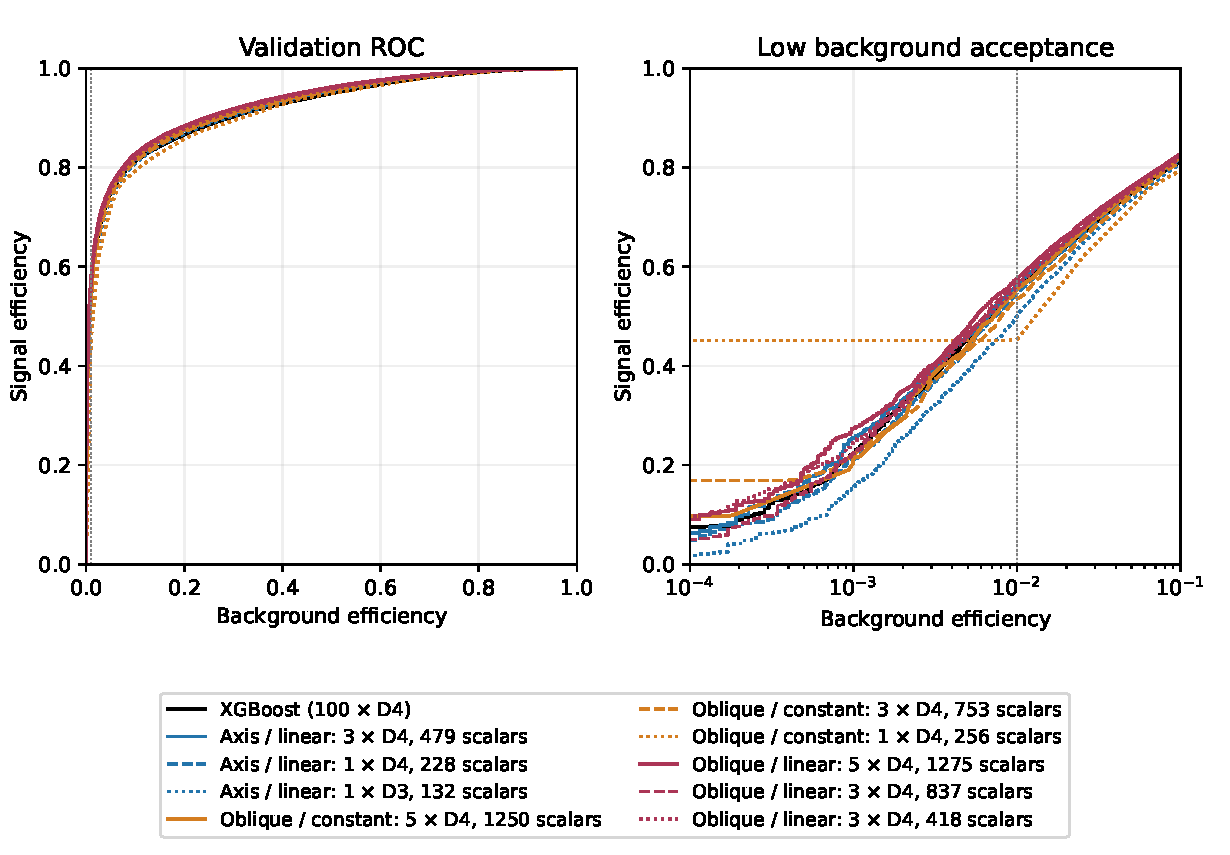
\includegraphics[width=\textwidth]{figures/family_roc.pdf}
\caption{The ten selected configurations on the same validation partition.
Colors identify families; line styles distinguish their representatives.
The low-background panel resolves the primary working point.
Numbers in the legend are learned nonzero scalar counts, with the axis-cut
storage convention defined in the text.}
\label{fig:families}
\end{figure}

Linear leaf functions can compensate for a smaller or sparser partition.
Compact refit reaches 56.20\% with 418 nonzeros (379 after input-independent branch pruning), approximately three times
fewer than the 1250-coefficient constant-leaf winner. This comparison includes
both cut and leaf coefficients: a richer leaf increases its own arithmetic,
but can reduce the overall number of retained cuts and weights. Conversely,
axis-aligned routing can remain competitive when the leaves are expressive.
A single axis-aligned depth-four tree reaches 54.74\% using 228 learned
nonzero scalars and 15 feature choices/direction bits. Three such trees reach
56.32\% using 479 scalars and 45 discrete cut choices.

The distinction between interpolation and a realizable threshold matters most
for coarse constant-leaf scores. The constant-leaf winner's interpolated
55.40\% becomes 54.75\% at a strict threshold respecting the 525-background
event budget. The selected linear-leaf entries retain their displayed
working-point efficiencies under the strict-threshold convention. A high AUC
alone does not establish a better low-background selection. A strict threshold
is tied to its numerical evaluator: changing even binary64 reduction order can
move an event at the cut, so the working point must be checked again after a
change of arithmetic, not only after quantization.

\begin{figure}[htbp]\centering
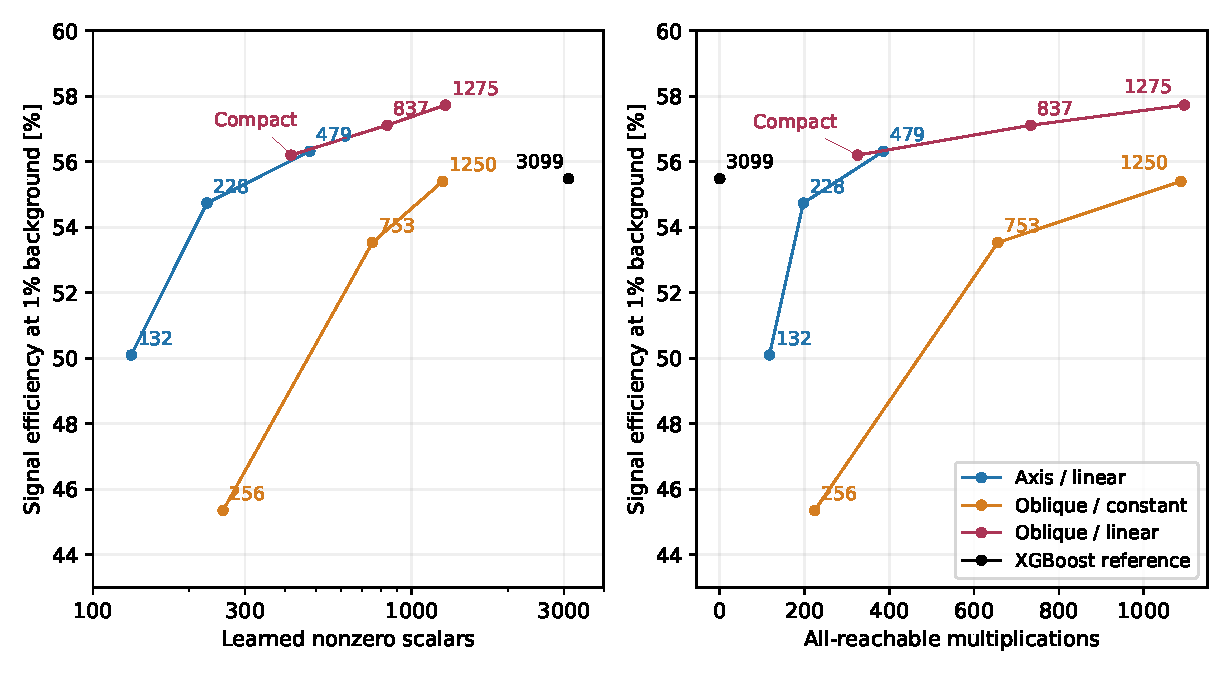
\includegraphics[width=\textwidth]{figures/family_tradeoff.pdf}
\caption{Representative validation operating points versus learned nonzero
scalars (left) and all-reachable multiplications after exact-zero/unit-factor
elimination (right). Lines only connect the selected representatives.
Labels identify scalar counts; Compact denotes the 418-coefficient refit.
Feature indices, direction bits, comparisons and additions are separate costs.
XGBoost uses no general multiplications here, but still performs tree decisions
and score aggregation.}
\label{fig:family-cost}
\end{figure}

\subsection{Matched CPU evaluation and arithmetic workload}
\label{sec:cost}
The C++ column in Table~\ref{tab:comparison} uses one common sparse path-traversal
reference for all ten models. Inputs and coefficients are binary64, with
XGBoost inputs rounded to binary32 before traversal to preserve its native
feature semantics. Exact-zero and unit-factor operations are eliminated;
axis cuts use direct comparisons. All node and coefficient structures are
loaded before timing. With one thread, one untimed warmup and nine timed
repeats of the full 132,800-event batch, we report median wall time divided
by event count. Parsing, preprocessing, allocation, input conversion and file
I/O are excluded. The measurement host is a KVM guest reporting Intel Xeon
Gold 6138 processors with a nominal 2.00 GHz clock; no fixed-frequency control
is assumed. Compilation uses GCC 12.3.1, C++17, optimization level 3 and disabled
fused multiply-add contraction. The results measure bulk throughput, not
single-event latency.

The axis three-tree depth-four model takes 0.101 microseconds per event,
compared with 0.167 for Compact refit, 0.412 for the five-tree oblique/linear
winner and 0.965 for the five-tree constant-leaf winner. The common reference
takes 3.675 microseconds for XGBoost. Separately, the optimized native XGBoost
library takes 1.478 microseconds per event on the same host and batch,
including probability output. Thus the common kernel is a controlled
reference, not the best achievable software implementation of every model.
Differences from earlier NumPy and C++ prototype timings must not be read as
changes in the algorithms' intrinsic cost.

The choice of hardware schedule changes the relevant arithmetic comparison.
Axis three-tree depth-four routing requires no general multiplications, and
its selected-path bound is 35 leaf products, versus 78 total products for
Compact refit. Computing all reachable affine functions instead requires 386
products for the axis model and 325 for Compact refit. Their path comparison
bounds are both 12. The axis model therefore has fewer sequential-path
products, but more scalars (479 versus 418), more all-node products and
additional discrete cut choices. Neither point uniformly dominates the other.
XGBoost has zero general products because the learning rate is absorbed into
its leaf values, yet has up to 400 path comparisons and 1499 internal decisions
in an all-node evaluation. Multiplication count alone cannot rank all designs.

\begin{implementation}
\textbf{One timing kernel and independent checks.}
\file{fpga/comparison/benchmark.cc} implements the shared sparse reference.
\file{scripts/run_ten_model_comparison.sh} uses the pinned EL9/CMSSW environment;
\file{scripts/compare_ten_models.py} prepares canonical models and validates
predictions and every leaf assignment before recording results (16.6 million assignments across
the ten validation predictions). The host was
\code{clip-c2-48.cbe.vbc.ac.at}, with GCC 12.3.1,
\code{-O3 -std=c++17 -ffp-contract=off}. All leaf assignments match exactly on
validation. The largest XGBoost margin difference from native inference is
$2.89\times10^{-6}$; each TAO margin differs by less than $10^{-9}$.
\code{operations} counts nonzero, non-unit feature factors after constant-route
pruning. Older \code{sparsity_profile} counts retain unit products and are
therefore slightly larger; the final table uses the new convention consistently.
\file{paper/build_comparison_assets.py} regenerates the table from the frozen
report; \code{--plot} additionally needs archived validation scores on CLIP.
\end{implementation}

\FloatBarrier
\section{Discussion and conclusions}
\label{sec:discussion}
The comparison supports three observations. First, expressive leaves can
reduce the total coefficient and arithmetic budget needed for a useful
working point. Compact refit's 418 scalars reach comparable validation
performance to the 3099-scalar boosted reference, and exceed the selected
1250-scalar constant-leaf forest's working point. Second, inexpensive axis
routing with linear leaves is competitive: the 479-scalar model reaches
56.32\%, while a single 228-scalar tree reaches 54.74\%. Third, the preferred
candidate depends on implementation schedule. For the two candidates near 56.2\%, the axis model uses fewer selected-path
products; Compact refit uses fewer scalars and fewer all-node products. The larger
oblique/linear model supplies the highest observed working point, 57.73\%,
at a higher resource budget. The final table records these distinct choices.

No single scalar count captures FPGA cost. Fixed unit cuts, nontrivial affine
weights, comparisons, adders, sparse indices and leaf selection differ in
implementation cost. Zero products do not make XGBoost free: its tree count
still requires substantial routing and score aggregation. A path evaluator
can reuse arithmetic but has sequential dependencies; an all-node pipeline
can spend more resources to expose parallelism. Coefficient precision and
constant-multiplier transformations can change either ranking. C++ throughput
is useful software evidence, but does not determine FPGA clock, initiation
interval or latency.

Training and selection also limit interpretation. The common objective and
fixed data partitions support a consistent candidate comparison, but the
families have different scan and refitting histories. \SFR{} can recover
shrinkage loss without restoring excluded directions; it cannot repair an
inadequate selected support. Axis three-tree depth-three performance is worse
at the primary working point than a smaller single depth-four tree, despite
its slightly higher AUC. Model size is not a guarantee of low-background
performance. Separation explains why one unpenalized axis refit was held,
rather than being reported as a converged improvement. Existing conditional
bootstrap intervals for the earlier subset are retained in
Appendix~\ref{app:uncertainty}; no independent significance claim is made for
the small differences between the new selected models.

This closes the floating-point candidate comparison and its supporting
numerical implementation checks. Hardware evaluation requires a common target
device, clock, interface and throughput requirement; validated feature,
coefficient and accumulator formats; and a recalibrated realizable selection
threshold after quantization. The scalar-leaf weighted-cut implementation is
already numerically checked, whereas affine leaves require a corresponding
hardware-backend extension. Synthesis must decide whether simpler routing or
sparser all-node computation provides the better resource/latency tradeoff.
Further test evaluation should retain disclosure of the historical XGBoost-only
test check and use model choices fixed before inspecting that partition.

\begin{implementation}
\textbf{Final handover.} \file{fpga_handoff/CURRENT_COMPARISON.json} pins
\file{fpga_handoff/comparison_v1/manifest.json} and its verification report.
All ten table entries have exact standardized coefficients, golden vectors,
metrics and training/configuration pointers. The three family winners and
Compact refit have distinct roles; no synthesized hardware winner is selected.
\file{docs/DORIAN_HANDOVER.md} is the entry point for Dorian.
The historical v3 bundle and its default remain reproducible.
\end{implementation}

\FloatBarrier
\bibliographystyle{unsrtnat}
\bibliography{references}
\clearpage
\appendix
\section{Support-selection and refit results}
\label{app:support}
For Compact refit, a converged three-tree parent was continued along a
split-penalty path
$\lambda_s=3\cdot10^{-5},10^{-4},3\cdot10^{-4},10^{-3},3\cdot10^{-3}$,
with $\lambda_\ell=10^{-5}$. The terminal fit at the final penalty supplied
418 coefficients. Leaf-only refitting raised validation efficiency from
54.59\% to 54.81\%. Full alternating refitting converged after 15 epochs at
55.98\%; its best saved validation snapshot was epoch 8 at 56.20\%. The
selected model is this earlier snapshot, with the same 418 coefficients.
An additional one-tree oblique reference, retained in the historical uncertainty
subset but not among the final ten representatives, was trained without L1
and without SFR.

Table~\ref{tab:sfr} and Fig.~\ref{fig:tradeoff} summarize ten parent supports.
Six full refits completed, two were held for separation and two for an
inconclusive linear-program timeout. The higher-efficiency model is a completed
leaf-only refit at 57.12\%, improving its own parent by about 0.21 percentage
points. Its full stage was held and is excluded from selection. Stronger
penalization does not consistently improve the accuracy--size tradeoff;
refitting cannot restore a direction removed by support selection.

\begin{table}[htbp]\centering\small
\caption{Fixed-support refitting study. Efficiencies are percentages at 1\%
background. All models have three depth-four trees except the starred
one-tree case. Parent and leaf columns are terminal stage results; best is the
best eligible saved leaf/full refit. Held full stages contribute no candidates.
The support budget is the parent's exact nonzero count.}
\label{tab:sfr}\setlength{\tabcolsep}{4pt}
\begin{tabular}{@{}lrrrrl@{}}\toprule
$\lambda_s/\lambda_\ell$ & Support & Parent & Leaf & Best & Full stage\\\midrule
0.0001/0.0001 & 520 & 55.58 & 55.82 & 56.49 & complete \\
0.0003/1e-5 & 675 & 56.98 & 56.74 & 56.74 & timeout \\
1e-5/3e-5 & 837 & 56.91 & 57.12 & 57.12 & timeout \\
0.0003/0.0003 & 394 & 54.48 & 54.85 & 54.85 & separated \\
1e-5/1e-5$^*$ & 403 & 55.20 & 55.06 & 55.08 & complete \\
0.001/1e-5 & 561 & 56.06 & 56.32 & 56.46 & complete \\
3e-5/3e-5 & 777 & 56.62 & 56.75 & 56.75 & complete \\
1e-5/1e-5 & 889 & 56.40 & 56.45 & 56.74 & complete \\
0.003/1e-5 & 418 & 54.59 & 54.81 & 56.20 & complete \\
0.001/0.001 & 317 & 51.27 & 52.52 & 52.52 & separated \\
\bottomrule
\end{tabular}
\end{table}

\begin{figure}[H]\centering
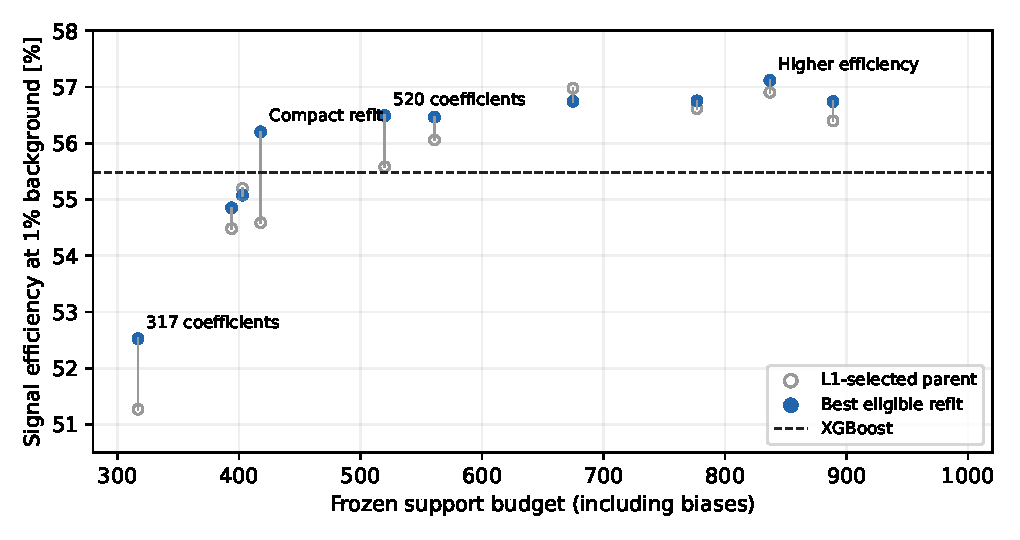
\includegraphics[width=\textwidth]{figures/sfr_research.pdf}
\caption{L1-selected terminal parents and their best eligible fixed-support
refits. Each vertical segment keeps the support budget fixed. Only refits
from eligible stages contribute; the penalty settings are given in
Table~\ref{tab:sfr}.}
\label{fig:tradeoff}
\end{figure}

\begin{implementation}
\textbf{Historical refit inputs.} This supporting study uses the v3 model bundle.
\file{fpga_handoff/CURRENT_MODEL.json} selects
\code{fpga_handoff/v3/compact_refit_3t_d4/}. The 837-coefficient alternative is
\code{highest_efficiency_3t_d4}; the one-tree reference is
\code{single_tree_1t_d4}. All exact source snapshots and masks are recorded
in the handover manifest. A later 57.24\% full-refit diagnostic for the
higher-efficiency support is held and not an eligible model.

\textbf{Compact training chain.} Start from the v2 \code{winner_3t_d4}
coefficients, run \file{configs/l1_path_v1/control.json}, then the split path
\code{split_01.json} through \code{split_05.json} in \code{configs/l1_path_v1/}.
The manifest is \file{configs/tao_l1_path_v1.json}. The final terminal parent
feeds \file{configs/support_refit_scan_v1/split300.json}. Parent training uses
\file{scripts/train_tao_fully.py}; SFR uses
\file{scripts/train_tao_support_refit.py},
\file{scripts/run_support_refit_scan_case.py} and
\file{scripts/support_refit_artifacts.py}. Exact refit reproduction begins with
the archived hash-pinned terminal parent, rather than a fresh fit at the final
penalties. The selected checkpoint hash is
\begin{center}\scriptsize\ttfamily\CompactCheckpointHash\end{center}

\textbf{Budgets.} The penalty path starts with local/joint/split iteration
budgets 300/250/300 and logs repeated chunks or adaptive increases. Compact
refit uses 400/400/800, L-BFGS-B tolerances \code{ftol=1e-12},
\code{gtol=1e-8}, at most 100 joint-fit chunks and 200 epochs per stage.
A 2,700-second allocation checkpoints with return code 75. A mild-control
router required a documented 800-to-4,000 iteration-budget amendment and
converged after 2,028 auxiliary iterations; this changed no objective or
stopping tolerances. See \file{scripts/amend_support_solver_budget.py} and
\file{docs/support_refit_scan_budget_amendments.json}.

\textbf{Snapshot layers.} The refit study was frozen on 25 October 2026.
The final comparison is separately frozen on 29 October and includes the
newly converged five-tree architecture winner at 57.73\%. Historical dated
records are retained but do not supersede this comparison.
\file{src/tao/uncertainty.py} supplies the earlier bootstrap;
\file{scripts/build_paper_inputs.py} regenerates that frozen supporting subset.
\end{implementation}

\FloatBarrier
\section{Axis-aligned linear-leaf cohort}
\label{app:axis}
All four CART-initialized source configurations converged under the common
objective/KKT/routing stability rules, with $\lambda_\ell=10^{-5}$ and
$\lambda_s=0$. Their frozen-support, fixed-cut unpenalized leaf refits produced
three converged stages and one separation outcome. Table~\ref{tab:axis-cohort}
reports the best eligible checkpoint for each layout. The three-tree depth-four
entry therefore uses its regularized source, and the three-tree depth-three
entry also retains its regularized checkpoint because its eligible refit did
not improve the primary validation metric.

\begin{table}[htbp]\centering\small
\caption{Complete axis/linear cohort. Scalar slots exclude fixed unit routing
weights; nonzeros include learned leaf values and active thresholds. Index
counts require an additional direction bit per nonconstant cut. The refit
column reports the unpenalized stage's outcome, not the source's convergence.}
\label{tab:axis-cohort}\setlength{\tabcolsep}{4pt}
\begin{tabular}{@{}lrrrrrl@{}}\toprule
Layout & Scalar slots & Nonzeros & Indices & $\epsilon_s$ [\%] & AUC & Refit\\\midrule
1$\times$D3 & 143 & 132 & 7 & 50.10 & 0.92020 & complete \\
1$\times$D4 & 287 & 228 & 15 & 54.74 & 0.92387 & complete \\
3$\times$D3 & 429 & 274 & 21 & 53.83 & 0.92414 & complete \\
3$\times$D4 & 861 & 479 & 45 & 56.32 & 0.92576 & separated \\
\bottomrule
\end{tabular}
\end{table}
A separated unpenalized fit is held because coefficients can grow along a
recession direction without a finite minimizing parameter vector, as described
in Section~\ref{sec:sfr}. Its regularized source can remain a valid
candidate; the held stage supplies no selected result.

\begin{implementation}
Exact source/refit states, selected epochs, hashes and parameter counts are in
\file{docs/axis_linear_v1/status.json}; the frozen paper copy is
\code{paper/sources/axis_linear_study.json}. The four source policies are
\code{configs/axis_linear_v1/case_0.json} through \code{case_3.json}; their
hash-pinned terminal parents feed \code{refit_0.json} through \code{refit_3.json}.
\file{scripts/monitor_axis_study.py} resumed only clean wall-time exits and
stopped when every case had a converged or explicitly held refit outcome.
No source in this four-case study remains incomplete.
\end{implementation}

\FloatBarrier
\subsection{Constant-leaf forests}
\label{sec:constant}
Constant predictions simplify the hardware leaf stage and permit comparison
with scalar-leaf FPGA tree architectures~\cite{conifer2020}. To study the
accuracy cost, we scan $T\in\{1,3,5\}$ trees, $D\in\{2,3,4\}$ and
$\lambda_s\in\{0,10^{-7},10^{-5}\}$, giving 27 configurations. Each uses the
same CART initialization seed, training partition and numerical stopping rules
as the factorial architecture study. Constant leaves have no feature weights,
so their nominal leaf penalty does not affect Eq.~\eqref{eq:objective}.
We select the saved checkpoint with the highest validation efficiency at
1\% background from each converged source run, and then select among
penalties for each layout.

\ifnum\ConstantCompleted<\ConstantTotal\relax
At this snapshot, \ConstantCompleted{} of \ConstantTotal{} source runs have
converged. The remaining five-tree, depth-four run with $\lambda_s=10^{-7}$
is still training and contributes no selected result. Table~\ref{tab:constant}
therefore reports the best eligible completed case per layout.
\else
All \ConstantTotal{} source runs have converged.
Table~\ref{tab:constant} reports the best selected penalty per layout.
\fi
The interpolated efficiency follows the common ROC convention. We also report
a strict threshold on the binary64 signal margin that accepts at most 525
background events. This distinction matters for shallow constant trees:
a single depth-$D$ tree has at most $2^D$ score levels, and even its highest
level can exceed the background budget. Connecting ROC vertices then gives
an interpolated efficiency that a deterministic threshold cannot realize.

\begin{table}[htbp]\centering\small
\caption{Constant-leaf forests: the best eligible penalty per layout.
$\epsilon_s$ is interpolated at 1\% background; $\epsilon_s^{\rm strict}$ uses
a realizable strict margin threshold with background efficiency at most 1\%.
Both coefficient counts include biases.}
\label{tab:constant}\setlength{\tabcolsep}{4pt}
\begin{tabular}{@{}lrrrrrr@{}}\toprule
Layout & $\lambda_s$ & $P_{\rm dense}$ & $P_{\rm nz}$ & $\epsilon_s$ [\%] & $\epsilon_s^{\rm strict}$ [\%] & AUC\\\midrule
1 $\times$ D2 & $10^{-7}$ & 55 & 55 & 14.98 & 0.00 & 0.88179 \\
1 $\times$ D3 & $10^{-5}$ & 127 & 126 & 38.61 & 0.00 & 0.90357 \\
1 $\times$ D4 & 0 & 271 & 256 & 45.36 & 45.33 & 0.91247 \\
3 $\times$ D2 & $10^{-5}$ & 165 & 129 & 30.72 & 0.00 & 0.90087 \\
3 $\times$ D3 & 0 & 381 & 336 & 49.01 & 38.81 & 0.91763 \\
3 $\times$ D4 & 0 & 813 & 753 & 53.54 & 53.30 & 0.92318 \\
5 $\times$ D2 & $10^{-7}$ & 275 & 275 & 47.77 & 47.01 & 0.91283 \\
5 $\times$ D3 & $10^{-7}$ & 635 & 615 & 50.94 & 50.31 & 0.92176 \\
5 $\times$ D4 & 0 & 1355 & 1250 & 55.40 & 54.75 & 0.92610 \\
\bottomrule
\end{tabular}
\end{table}

The selected constant configuration has \ConstantWinnerTrees{} trees of
depth \ConstantWinnerDepth{}, with \ConstantWinnerNonzero{} nonzeros in
\ConstantWinnerDense{} allocated slots. It reaches
\ConstantWinnerEfficiency\% interpolated signal efficiency; its realizable
strict-threshold efficiency is \ConstantWinnerStrict\%.
Figure~\ref{fig:constant} compares the depth-four constant forests with XGBoost
and the sparse linear-leaf Compact refit. These are comparisons of selected
configurations: their penalty and refitting histories differ, so the comparison
is not a leaf-type ablation at identical support.
\begin{figure}[htbp]\centering
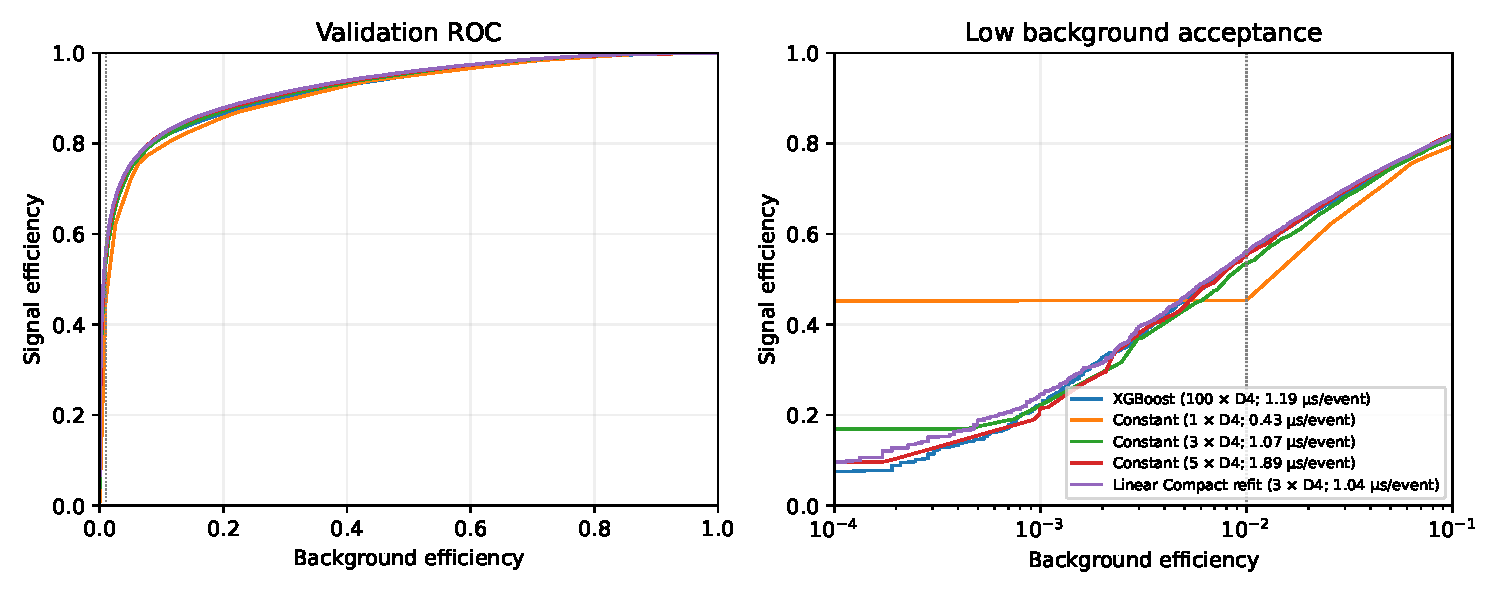
\includegraphics[width=\textwidth]{figures/constant_leaf_roc.pdf}
\caption{Validation ROCs for the best completed constant-leaf configuration at
each depth-four layout, compared with XGBoost and linear-leaf Compact refit.
The low-background panel exposes the coarse score steps of small constant
forests. Eligibility requires convergence of the source run; selection can
choose an earlier saved epoch. Parenthetical times are bulk CPU wall time per
event on the 132,800-event batch: one thread, median of nine repeats. TAO uses
the NumPy prediction API on binary64 inputs and XGBoost uncached compiled
prediction on preconverted binary32 inputs. These follow-up measurements are separate from Table~\ref{tab:main}
and are not FPGA or single-event latency.}
\label{fig:constant}
\end{figure}
\FloatBarrier

For these candidates, linear predictions reduce the number of nonzero
coefficients from 1250 to 418, a factor of 2.99, while increasing the
interpolated signal efficiency from 55.40\% to 56.20\%.
After eliminating only input-independent branches and exact-zero terms,
the respective all-node multiplication counts are 1095 and 327; selected-path
upper bounds are 275 and 80. The additional leaf arithmetic is therefore
more than offset by the sparser, smaller forest in this comparison.
These scalar operation counts do not determine synthesized resource use:
precision, scheduling, constant-multiplier optimization and storage layout
must also be specified.




A matched compiled sparse traversal provides an additional CPU check. With
one thread and the full 132,800-event validation batch, the median of nine
repeats after one warmup is \LeafConstantCPU{} microseconds per event for
the constant forest and \LeafLinearCPU{} for the linear forest.
Both use binary64 arithmetic and the same traversal strategy; input conversion
and file I/O are excluded. These are CPU batch measurements, with no inference
about FPGA latency.

For an exploratory reduced-precision comparison, each cut is first multiplied
by a positive power of two, $w'_{tv}=2^{k_{tv}}w_{tv}$ and
$b'_{tv}=2^{k_{tv}}b_{tv}$. This preserves its real-arithmetic decision; the
exported binary64 scaling is constrained to retain every nonzero coefficient,
and validation leaf assignments are checked before quantization.
We use the nearest-even, saturating quantizer of Eq.~\eqref{eq:quantizer}, with
10 integer bits for inputs, thresholds and cut accumulators, 6 for weights,
and 16 for scores and leaf biases, all including sign. Every type uses the
same fractional width $F$. Cast inputs and coefficients precede multiplication;
cut products accumulate in feature order, with a cast to the cut-accumulator
format after each addition. For a linear leaf, products accumulate similarly
in the score format, followed by the leaf bias. The negative tree outputs are
summed in the score format. Integer widths are conservatively checked against
absolute partial-sum bounds in the observed training box; they have not been
minimized separately for the two candidates.

\begin{table}[htbp]\centering\small
\caption{Common-format fixed-point emulation of the two selected leaf
architectures. Efficiencies are percentages at 1\% background. Total widths
are $F+10$ input/threshold bits, $F+6$ weight bits and $F+16$ score bits.}
\label{tab:leafprecision}
\begin{tabular}{@{}lrrr@{}}\toprule
Leaf type & $F$ & $\epsilon_s$ [\%] & $\epsilon_s^{\rm strict}$ [\%]\\\midrule
Constant & 18 & 55.40 & 54.75 \\
Constant & 12 & 55.40 & 54.75 \\
Constant & 8 & 55.18 & 54.38 \\
Linear & 18 & 56.20 & 56.20 \\
Linear & 12 & 56.21 & 56.21 \\
Linear & 8 & 56.00 & 56.00 \\
\bottomrule
\end{tabular}
\end{table}
At $F=12$, both architectures remain within 0.02 percentage points of their
floating-point interpolated working-point efficiency (Table~\ref{tab:leafprecision}).
For constant leaves, independent fixed-point path traversal and the existing
weighted-cut backend agree exactly on all validation scores. The generated
all-node HLS C++ implementation also agrees exactly on a 512-vector check at
$F=12$. The linear-leaf evaluation uses an independent affine-leaf reference;
a corresponding HLS backend extension and synthesis remain to be completed.
These checks establish numerical feasibility at common precision, rather than
an optimized FPGA resource comparison.

\begin{implementation}
\textbf{Controlled cohort and exact snapshots.}
The constant subset of \file{configs/tao_hyper_scan_v1.json} comprises cases
3--5, 9--11, 15--17, 21--23, 27--29, 33--35, 39--41, 45--47 and 51--53.
These use CART initialization and hard-threshold search. They are separate
from the earlier seven-layout, randomly initialized constant study.
\file{scripts/build_constant_leaf_study.py} re-evaluates eligible checkpoints,
archives them under \code{models/constant_study_v1_selected/<sha256>.pkl},
and records selected and terminal epochs, metrics, configurations, convergence
checks and hashes in \code{paper/sources/constant_leaf_study.json}.
The selected constant model is also exported in
\code{paper/sources/constant_leaf_winner.json}; this does not alter the v3
handover or its default. Its selected epoch is \ConstantWinnerEpoch{}, while
the source run terminates at epoch \ConstantWinnerTerminalEpoch{}.

Regenerate with the pinned training environment:
\begin{lstlisting}[language=bash]
PYTHONPATH=src:. python scripts/build_constant_leaf_study.py
# Final gate: exits unsuccessfully while any source case is incomplete.
PYTHONPATH=src:. python scripts/build_constant_leaf_study.py --require-complete
\end{lstlisting}
The two-candidate entry point is
\file{fpga_handoff/CURRENT_CANDIDATES.json}. The constant winner is frozen in
\code{fpga_handoff/leaf_competition_v1/constant_5t_d4/}; the linear candidate
points to the unchanged v3 Compact refit. Both input spaces have canonical
JSON, hexadecimal coefficients and golden vectors.
\file{docs/leaf_competition_v1/README.md} records CPU/precision results and
\file{scripts/run_leaf_competition.sh} reproduces them in the pinned EL9
container. The scalar-leaf adapter uses unmodified conifer 1.11; the CMSSW
1.7 external cannot evaluate oblique weights. The affine-leaf reference is
\file{fpga/leaf_competition/emulate.cc}, not a conifer HLS backend extension.
\file{scripts/verify_fpga_handoff.py} checks both candidates and both input
spaces without a Python training stack.

Training compute times and both probability-based and binary64-margin strict
working points are retained in the snapshot and
\file{docs/constant_leaf_study_v1.md}. Incomplete cases remain visible and are
never labelled converged or promoted into the table.
\end{implementation}

\FloatBarrier
\section{Fixed-point feasibility checks}
\subsection{A fixed-point XGBoost reference}
\label{sec:fixedpoint}
As a first numerical implementation check, we emulate the XGBoost reference
with signed fixed-point inputs, thresholds and scores. A format with total
width $W_b$ and integer width $I_b$ has $F_b=W_b-I_b$ fractional bits and
representable range
$[-2^{I_b-1},\,2^{I_b-1}-2^{-F_b}]$. Define its quantizer by
\begin{equation}
 Q_{W_b,I_b}(u)=\operatorname{clip}_{W_b,I_b}
 \!\left(2^{-F_b}\operatorname{round}_{\rm even}(2^{F_b}u)\right),
 \label{eq:quantizer}
\end{equation}
where rounding chooses the nearest integer with ties to even, and clipping
saturates at the format's endpoints. We quantize inputs and thresholds before
evaluating the strict-left XGBoost cuts. Let $s_{t\ell}$ denote a scalar leaf contribution with the learning rate
absorbed, and $s_0$ the initial margin. These values
use the score format; tree scores are combined by a balanced adder tree with
casts to that format after additions. Its result is added to the quantized
initial margin and cast once more. No sigmoid is needed for selection.

The maximum absolute training input is 8.96 and the largest absolute tree
threshold is 4.73, so we use $I_b=5$ for inputs and thresholds. For the
$T=100$ tree scores, define
\begin{equation}
 A=|s_0|+\sum_{t=1}^{T}\max_\ell|s_{t\ell}|\simeq15.09.
 \label{eq:score-bound}
\end{equation}
At the coarsest fractional width $F_{\min}=4$, rounding the $T$ leaf values
and initial margin can add at most $(T+1)2^{-F_{\min}-1}$ to this bound.
Their quantized sum and all partial sums therefore fit within an absolute
bound of 18.25, covered by $I_b=6$ for scores. With no overflow, sums of values
on this common fixed-point grid introduce no further fractional rounding.
No validation input lies outside the chosen input range. We vary the common
fractional width while keeping these integer widths fixed. Table~\ref{tab:fixedpoint}
shows the resulting validation performance. The 17/18-bit input/score pair
retains the reference working-point efficiency; the coarsest 9/10-bit pair
loses performance and produces more substantial score ties. Small positive
changes in the interpolated point are not interpreted as an established
accuracy gain.

\begin{table}[htbp]\centering\small
\caption{XGBoost fixed-point emulation on the same validation partition.
Widths include the sign bit; input and threshold formats are identical.
The native reference has $\epsilon_s=55.48\%$ and AUC 0.92056.
The strict-threshold column uses background efficiency at most 1\%.}
\label{tab:fixedpoint}\setlength{\tabcolsep}{5pt}
\begin{tabular}{@{}rrrrr@{}}\toprule
Input bits & Score bits & $\epsilon_s$ [\%] & $\epsilon_s^{\rm strict}$ [\%] & AUC\\\midrule
23 & 24 & 55.48 & 55.48 & 0.92056 \\
17 & 18 & 55.49 & 55.49 & 0.92056 \\
15 & 16 & 55.46 & 55.45 & 0.92056 \\
13 & 14 & 55.56 & 55.53 & 0.92048 \\
11 & 12 & 55.47 & 55.29 & 0.92040 \\
9 & 10 & 52.05 & 50.85 & 0.91760 \\
\bottomrule
\end{tabular}
\end{table}
Independent C++ executions agree exactly for the tested fixed-point outputs.
This establishes numerical agreement of the emulators; FPGA resource use,
latency and initiation interval require synthesis for a specified device,
clock and interface.

\begin{implementation}
\textbf{Tested chain.} \file{docs/conifer_xgboost_v1/README.md} specifies the
EL9 container, CMSSW workspace, dependency pins and commands. Conversion and
HLS C++ generation use conifer 1.11; the axis-aligned reference is also evaluated
with the actual CMSSW conifer 1.7 external. Its bridge rejects oblique weights.
The full validation compares 13,280,000 native/exported leaf IDs, plus boundary
checks. Each of eight C++ profiles is checked on 512 HLS vectors, including all
324 frozen XGBoost handover vectors. Every fixed-point comparison is exact.
\file{fpga/conifer/compat.py} reconciles native binary32 thresholds, leaf
values, initial margin and actual depth; upstream conversion is retained
as a diagnostic. It is important to preserve XGBoost's input rounding and
strict-left equality convention. The score-type settings in the table are
\code{AP_RND_CONV, AP_SAT}; axis weights are exact one-hot constants.

\file{docs/conifer_xgboost_v1/validation.json} contains full provenance and
per-profile metrics. \file{scripts/validate_xgboost_conifer.py} reads training
inputs for range selection and validation arrays for evaluation; test arrays
are not loaded. Generated projects use conifer's default device/clock only as
export placeholders. No FPGA synthesis has been run, and CPU timings that
include file I/O are not reported as hardware latency.
\end{implementation}

\FloatBarrier
\subsection{Oblique-leaf feasibility check}
The following supporting precision check concerns the previously frozen
five-tree constant-leaf winner and three-tree linear Compact refit only.
It does not quantize all ten final representatives or the new axis/linear cohort.
For an exploratory reduced-precision comparison, each cut is first multiplied
by a positive power of two, $w'_{tv}=2^{k_{tv}}w_{tv}$ and
$b'_{tv}=2^{k_{tv}}b_{tv}$. This preserves its real-arithmetic decision; the
exported binary64 scaling is constrained to retain every nonzero coefficient,
and validation leaf assignments are checked before quantization.
We use the nearest-even, saturating quantizer of Eq.~\eqref{eq:quantizer}, with
10 integer bits for inputs, thresholds and cut accumulators, 6 for weights,
and 16 for scores and leaf biases, all including sign. Every type uses the
same fractional width $F$. Cast inputs and coefficients precede multiplication;
cut products accumulate in feature order, with a cast to the cut-accumulator
format after each addition. For a linear leaf, products accumulate similarly
in the score format, followed by the leaf bias. The negative tree outputs are
summed in the score format. Integer widths are conservatively checked against
absolute partial-sum bounds in the observed training box; they have not been
minimized separately for the two candidates.

\begin{table}[htbp]\centering\small
\caption{Common-format fixed-point emulation of the two selected leaf
architectures. Efficiencies are percentages at 1\% background. Total widths
are $F+10$ input/threshold bits, $F+6$ weight bits and $F+16$ score bits.}
\label{tab:leafprecision}
\begin{tabular}{@{}lrrr@{}}\toprule
Leaf type & $F$ & $\epsilon_s$ [\%] & $\epsilon_s^{\rm strict}$ [\%]\\\midrule
Constant & 18 & 55.40 & 54.75 \\
Constant & 12 & 55.40 & 54.75 \\
Constant & 8 & 55.18 & 54.38 \\
Linear & 18 & 56.20 & 56.20 \\
Linear & 12 & 56.21 & 56.21 \\
Linear & 8 & 56.00 & 56.00 \\
\bottomrule
\end{tabular}
\end{table}
At $F=12$, both architectures remain within 0.02 percentage points of their
floating-point interpolated working-point efficiency (Table~\ref{tab:leafprecision}).
For constant leaves, independent fixed-point path traversal and the existing
weighted-cut backend agree exactly on all validation scores. The generated
all-node HLS C++ implementation also agrees exactly on a 512-vector check at
$F=12$. The linear-leaf evaluation uses an independent affine-leaf reference;
a corresponding HLS backend extension and synthesis remain to be completed.
These checks establish numerical feasibility at common precision, rather than
an optimized FPGA resource comparison.


\begin{implementation}
\file{docs/leaf_competition_v1/README.md} records this earlier two-candidate
experiment. \file{scripts/run_leaf_competition.sh} and
\file{fpga/leaf_competition/emulate.cc} reproduce its independent sparse
reference. Constant leaves use unmodified conifer 1.11 weighted-cut/scalar-leaf
backends; the old CMSSW 1.7 external is axis-aligned only. Affine leaves still
require a conifer HLS backend extension. This feasibility check is separate
from the final common timing kernel and does not establish synthesized resources.
\end{implementation}

\FloatBarrier
\section{Conditional uncertainty of an earlier subset}
\label{app:uncertainty}
These previously frozen intervals concern Compact refit, the 837-coefficient
leaf refit and a one-tree oblique reference. They are not intervals for all ten
current representatives; in particular they do not assess the new axis/linear
models or five-tree performance winner. In this supporting table, ``Higher
efficiency denotes the 837-coefficient refit.

A paired class-stratified bootstrap with 1,000 replicates, seed 20261025,
recomputes the interpolated working point in each replicate.
Table~\ref{tab:uncertainty} gives percentile intervals for the difference from
XGBoost. The Compact interval includes zero. These intervals condition on the
selected models and account for neither hyperparameter/checkpoint selection
nor training-seed variation; they are not independent test claims.
\begin{table}[H]\centering\small
\caption{Conditional validation efficiency difference from XGBoost, in
percentage points (pp), with paired 95\% percentile intervals.}
\label{tab:uncertainty}
\begin{tabular}{@{}lrr@{}}\toprule
Model & Difference [pp] & Interval [pp]\\\midrule
Compact refit & +0.72 & [-0.43, +1.52] \\
Higher efficiency & +1.63 & [+0.65, +2.55] \\
One-tree reference & +0.15 & [-1.08, +0.97] \\
\bottomrule
\end{tabular}
\end{table}

\FloatBarrier
\Needspace{16\baselineskip}
\section{Input feature order}
\label{app:features}
Table~\ref{tab:features} defines the coordinates $r_f$ of the archived feature
vector, using the source dataset's feature names. All displayed cuts use their
standardized counterparts $x_f$ from Eq.~\eqref{eq:standardization}.
\begin{table}[H]\centering\small
\caption{Feature-coordinate convention. Names identify columns in the
high-level jet dataset~\cite{openml42468}.}\label{tab:features}
\begin{tabular}{@{}rlrl@{}}\toprule
$f$ & Dataset feature & $f$ & Dataset feature\\\midrule
1 & \texttt{zlogz} & 9 & \texttt{d2\_a1\_b1\_mmdt}\\
2 & \texttt{c1\_b0\_mmdt} & 10 & \texttt{d2\_a1\_b2\_mmdt}\\
3 & \texttt{c1\_b1\_mmdt} & 11 & \texttt{m2\_b1\_mmdt}\\
4 & \texttt{c1\_b2\_mmdt} & 12 & \texttt{m2\_b2\_mmdt}\\
5 & \texttt{c2\_b1\_mmdt} & 13 & \texttt{n2\_b1\_mmdt}\\
6 & \texttt{c2\_b2\_mmdt} & 14 & \texttt{n2\_b2\_mmdt}\\
7 & \texttt{d2\_b1\_mmdt} & 15 & \texttt{mass\_mmdt}\\
8 & \texttt{d2\_b2\_mmdt} & 16 & \texttt{multiplicity}\\\bottomrule
\end{tabular}
\end{table}

\FloatBarrier
\section{Actual learned functions}
\label{sec:example}
Actual cuts illustrate the mixture of axis-aligned, oblique and constant
nodes. In Compact refit, using the standardized feature indices of
Table~\ref{tab:features}, the first tree contains
\begin{equation}\begin{aligned}
h_{1,\varnothing}(x)&\simeq x_{4} + 0.4216204
\end{aligned}\label{eq:example-root}\end{equation}
\begin{equation}\begin{aligned}
h_{1,L}(x)&= 0
\end{aligned}\label{eq:example-constant}\end{equation}
\begin{equation}\begin{aligned}
h_{1,R}(x)&\simeq 0.088106595x_{4} + 0.0025365055x_{6} + 0.17735909x_{11}\\
&\quad + 0.031223362x_{15} + 0.10064081x_{16} + 0.019058664
\end{aligned}\label{eq:example-oblique}\end{equation}

Coefficients marked $\simeq$ are rounded to eight significant digits. At the
root an event goes right if $x_4>-0.4216204$. Otherwise it reaches $L$, whose
constant cut sends it left again. Hence the entire $LR$ subtree is
unreachable. The root's right child combines five input features.

For the second tree, another learned cut is
\begin{equation}h_{2,L}(x)\simeq -2.3776136\cdot10^{-11}x_{16} - 3.1703281\cdot10^{-11}\label{eq:example-tiny}\end{equation}

Its small scale does not make it uninformative: it routes right approximately
when $x_{16}<-1.3334$. Setting both coefficients to zero would turn it into a
constant left route. This example motivates distinguishing exact sparsity
from coefficient magnitude before quantization.

\begin{implementation}
\textbf{Print the actual functions.} \code{TreePrinter} in
\file{src/tao/printing.py} provides \code{print_tree}, \code{format_tree},
\code{format_forest} and \code{records}. The CLI
\file{scripts/print_tao_tree.py} prints every cut and affine leaf, including
unreachable branches. It is read-only and separate from pinned fitting code.
For example, after setting the environment described below:
\begin{lstlisting}[language=Python]
import json
from pathlib import Path
from tao.printing import TreePrinter
spec = json.loads(Path(
    "fpga_handoff/v3/compact_refit_3t_d4/standardized/model.json"
).read_text())
TreePrinter(spec, precision=17).print_tree(0)
\end{lstlisting}
The complete 17-digit record is
\code{generated/compact_forest_full_precision.txt}; the annotated supplement
prints all three trees at nine display digits. Only exact-zero terms are
omitted. Independent tests parse the printed expressions, recover all 418
nonzero coefficients, count 379 reachable coefficients, and compare predictions
with the portable evaluator. They also check equality routing, constant leaves,
tiny terms and non-mutation. The printer tests also preserve the source model and its exact-zero support.
\end{implementation}

\begin{implementation}

\textbf{Environment and entry points.}
Training and input regeneration use Python 3.10 with the pinned
\file{requirements.txt}: NumPy 1.26.4, SciPy 1.15.2, scikit-learn 1.7.2,
XGBoost 3.2.0, PyYAML 6.0.3 and matplotlib 3.10.7. The reference CLIP checkout
is \path{/users/robert.schoefbeck/CMS/tree_benchmark}; its Conda environment is
\code{tree-benchmark}. On CLIP use the conda-forge CPU XGBoost build, since the
PyPI Linux wheel requires newer glibc than the reference login environment.
No GPU is needed.
\begin{minipage}{\textwidth}
\begin{lstlisting}[language=bash]
source /software/f2022/software/mamba/24.3.0-0/etc/profile.d/conda.sh
conda activate tree-benchmark
cd /users/robert.schoefbeck/CMS/tree_benchmark
export PYTHONPATH="$PWD/src:$PWD" PYTHONDONTWRITEBYTECODE=1
export OMP_NUM_THREADS=1 OPENBLAS_NUM_THREADS=1 MKL_NUM_THREADS=1
python scripts/print_tao_tree.py \
  --model fpga_handoff/v3/compact_refit_3t_d4/standardized/model.json \
  --precision 17 --output /tmp/compact_forest.txt
\end{lstlisting}
\end{minipage}
For a new training account or checkout, the complete environment-creation and
controlled refit recipe is in \file{docs/DORIAN_HANDOVER.md}. The datasets and
pickle archives are deliberately not in Git. Exact reproduction of the refit
starts from the hash-pinned terminal parent; rebuilding its entire L1 path can
produce differently serialized checkpoint bytes and requires a new explicit
source hash/run name. Existing named runs must not be resumed under changed
training code or stopping policies. The standalone \code{paper/} folder,
however, contains all generated text/tables and figures needed to compile this
PDF without datasets, model pickles or a Python training environment.

\par\begingroup\small
\textbf{Implementation map.}\par\smallskip
\renewcommand{\arraystretch}{1.15}
\begin{tabularx}{\linewidth}{@{}p{.36\linewidth}X@{}}\toprule
Object / operation & Entry point\\\midrule
Axis cut search & \code{AxisTAOClassifier._split_update} in \file{src/tao/axis.py}\\
Matched C++ comparison & \file{fpga/comparison/benchmark.cc}; \file{scripts/compare_ten_models.py}\\
Final table generation & \file{paper/build_comparison_assets.py}\\
Routing, logits, objective & \code{HardTree}; \code{HardTAOClassifier} in \file{src/tao/hard.py}\\
Weighted leaf optimization & \code{fit_leaf_parameters}; \code{ce_value_gradient}\\
Joint leaf design/refit & \code{_joint_design}; \code{global_refit}\\
Reduced split proposals & \code{_hard_split_update}; \code{FrozenSupportTAO._split_update}\\
Sorted hard threshold search & \code{best_threshold} in \file{src/tao/split_search.py}\\
Node-resumable epoch & \code{begin_epoch}; \code{step_epoch} in \file{src/tao/epoch.py}\\
Masks and separation & \code{freeze_support}; \code{continue_full_refit}; \code{separation_check}\\
Stopping and exact-zero work counts & \code{leaf_kkt_residual}; \code{convergence_check}; \code{sparsity_profile}\\
Read-only equations & \code{TreePrinter.print_tree} in \file{src/tao/printing.py}\\
Portable inference / firmware export & \code{export_model}; \code{predict_margin}; \code{cpp_header} in \file{src/tao/portable.py}\\\bottomrule
\end{tabularx}
\par\endgroup

\textbf{Frozen coefficients and verification.}
\file{fpga_handoff/CURRENT_COMPARISON.json} pins all ten final entries in
\code{fpga_handoff/comparison_v1/}. Each TAO candidate has standardized
\code{model.json}, hexadecimal \code{model_coefficients.h}, ordered golden
inputs and expected margins/leaf indices. The bundle is standardized-only;
use its input contract and training scaler. Historical v3 additionally retains
raw-folded variants for its original candidates. Do not mix those input spaces.

\file{scripts/verify_comparison_handoff.py} needs Python's standard library and
a C++17 compiler. It checks every file hash, compiles the nine TAO references,
and independently walks exported XGBoost on its golden vectors. The full
common C++ benchmark separately checks every validation leaf assignment against
the canonical TAO or native XGBoost inference. Reproduction in a new checkout:
\begin{lstlisting}[language=bash]
python3 scripts/verify_comparison_handoff.py --compiler c++
# On CLIP, use EL9 because the native GCC is too old:
scripts/conifer_container.sh bash -c \\
 'source scripts/conifer_runtime.sh && workspaces/python/conifer/bin/python scripts/verify_comparison_handoff.py --compiler g++'
# Reproduce the measured comparison with archived data/checkpoints:
scripts/run_ten_model_comparison.sh
# Rebuild its document assets:
python3 paper/build_comparison_assets.py --plot
make -C paper
\end{lstlisting}
The plot command requires archived score files on CLIP; rebuilding both PDFs
from the complete \code{paper/} folder requires only TeX and the included
assets. \file{scripts/freeze_final_comparison.py} created the immutable bundle
once and refuses to overwrite it. The old model bundles, pointer and verification
reports remain available for historical reproduction. Fixed-point checks cover
the stated earlier subsets; no synthesis or full ten-model quantization claim
is made. Full training and configuration pointers are in
\file{docs/DORIAN_HANDOVER.md} and the new manifest.

\end{implementation}
\ifimplementationdetails
\clearpage
\section*{Implementation supplement: complete forest printout}
\begin{implementation}
This record is generated by \code{TreePrinter.format_tree} from the exact v3
standardized model. It lists every internal decision and every leaf output in
preorder, with heap indices and root-to-node paths. A node labelled unreachable
is excluded only by an input-independent constant ancestor, not by absent
training or validation examples. Numeric values are displayed with nine
significant digits. The full 17-digit record is checked in as
\path{generated/compact_forest_full_precision.txt}. These listings are for
inspection; implementation should consume the frozen JSON or hexadecimal
header. In all trees, a leaf output contributes to the background logit; the
signal margin is the \emph{negative sum} of the three selected outputs.


\textbf{Reading the record.} A path such as \code{RLLR} means right, left, left, right from the root. This path is the scientific node or leaf label. The extra \code{N} and \code{L} labels are internal-node and leaf-array indices; \code{heap} is a storage index. They have no mathematical role. Trees are numbered from zero in the file and from one in the scientific text.
\end{implementation}
\begin{implementation}
\textbf{Tree 0 (scientific tree $t=1$).}\par
\begingroup\setlength{\parskip}{0pt}
\noindent\begin{minipage}{\linewidth}
\lstinputlisting[style=treeblock,firstline=1,lastline=3]{generated/compact_tree_0.txt}
\end{minipage}\par
\noindent\begin{minipage}{\linewidth}
\lstinputlisting[style=treeblock,firstline=4,lastline=6]{generated/compact_tree_0.txt}
\end{minipage}\par
\noindent\begin{minipage}{\linewidth}
\lstinputlisting[style=treeblock,firstline=7,lastline=9]{generated/compact_tree_0.txt}
\end{minipage}\par
\noindent\begin{minipage}{\linewidth}
\lstinputlisting[style=treeblock,firstline=10,lastline=12]{generated/compact_tree_0.txt}
\end{minipage}\par
\noindent\begin{minipage}{\linewidth}
\lstinputlisting[style=treeblock,firstline=13,lastline=15]{generated/compact_tree_0.txt}
\end{minipage}\par
\noindent\begin{minipage}{\linewidth}
\lstinputlisting[style=treeblock,firstline=16,lastline=17]{generated/compact_tree_0.txt}
\end{minipage}\par
\noindent\begin{minipage}{\linewidth}
\lstinputlisting[style=treeblock,firstline=18,lastline=19]{generated/compact_tree_0.txt}
\end{minipage}\par
\noindent\begin{minipage}{\linewidth}
\lstinputlisting[style=treeblock,firstline=20,lastline=22]{generated/compact_tree_0.txt}
\end{minipage}\par
\noindent\begin{minipage}{\linewidth}
\lstinputlisting[style=treeblock,firstline=23,lastline=24]{generated/compact_tree_0.txt}
\end{minipage}\par
\noindent\begin{minipage}{\linewidth}
\lstinputlisting[style=treeblock,firstline=25,lastline=26]{generated/compact_tree_0.txt}
\end{minipage}\par
\noindent\begin{minipage}{\linewidth}
\lstinputlisting[style=treeblock,firstline=27,lastline=29]{generated/compact_tree_0.txt}
\end{minipage}\par
\noindent\begin{minipage}{\linewidth}
\lstinputlisting[style=treeblock,firstline=30,lastline=32]{generated/compact_tree_0.txt}
\end{minipage}\par
\noindent\begin{minipage}{\linewidth}
\lstinputlisting[style=treeblock,firstline=33,lastline=34]{generated/compact_tree_0.txt}
\end{minipage}\par
\noindent\begin{minipage}{\linewidth}
\lstinputlisting[style=treeblock,firstline=35,lastline=36]{generated/compact_tree_0.txt}
\end{minipage}\par
\noindent\begin{minipage}{\linewidth}
\lstinputlisting[style=treeblock,firstline=37,lastline=39]{generated/compact_tree_0.txt}
\end{minipage}\par
\noindent\begin{minipage}{\linewidth}
\lstinputlisting[style=treeblock,firstline=40,lastline=41]{generated/compact_tree_0.txt}
\end{minipage}\par
\noindent\begin{minipage}{\linewidth}
\lstinputlisting[style=treeblock,firstline=42,lastline=43]{generated/compact_tree_0.txt}
\end{minipage}\par
\noindent\begin{minipage}{\linewidth}
\lstinputlisting[style=treeblock,firstline=44,lastline=46]{generated/compact_tree_0.txt}
\end{minipage}\par
\noindent\begin{minipage}{\linewidth}
\lstinputlisting[style=treeblock,firstline=47,lastline=49]{generated/compact_tree_0.txt}
\end{minipage}\par
\noindent\begin{minipage}{\linewidth}
\lstinputlisting[style=treeblock,firstline=50,lastline=52]{generated/compact_tree_0.txt}
\end{minipage}\par
\noindent\begin{minipage}{\linewidth}
\lstinputlisting[style=treeblock,firstline=53,lastline=54]{generated/compact_tree_0.txt}
\end{minipage}\par
\noindent\begin{minipage}{\linewidth}
\lstinputlisting[style=treeblock,firstline=55,lastline=56]{generated/compact_tree_0.txt}
\end{minipage}\par
\noindent\begin{minipage}{\linewidth}
\lstinputlisting[style=treeblock,firstline=57,lastline=59]{generated/compact_tree_0.txt}
\end{minipage}\par
\noindent\begin{minipage}{\linewidth}
\lstinputlisting[style=treeblock,firstline=60,lastline=61]{generated/compact_tree_0.txt}
\end{minipage}\par
\noindent\begin{minipage}{\linewidth}
\lstinputlisting[style=treeblock,firstline=62,lastline=63]{generated/compact_tree_0.txt}
\end{minipage}\par
\noindent\begin{minipage}{\linewidth}
\lstinputlisting[style=treeblock,firstline=64,lastline=66]{generated/compact_tree_0.txt}
\end{minipage}\par
\noindent\begin{minipage}{\linewidth}
\lstinputlisting[style=treeblock,firstline=67,lastline=69]{generated/compact_tree_0.txt}
\end{minipage}\par
\noindent\begin{minipage}{\linewidth}
\lstinputlisting[style=treeblock,firstline=70,lastline=71]{generated/compact_tree_0.txt}
\end{minipage}\par
\noindent\begin{minipage}{\linewidth}
\lstinputlisting[style=treeblock,firstline=72,lastline=73]{generated/compact_tree_0.txt}
\end{minipage}\par
\noindent\begin{minipage}{\linewidth}
\lstinputlisting[style=treeblock,firstline=74,lastline=76]{generated/compact_tree_0.txt}
\end{minipage}\par
\noindent\begin{minipage}{\linewidth}
\lstinputlisting[style=treeblock,firstline=77,lastline=78]{generated/compact_tree_0.txt}
\end{minipage}\par
\noindent\begin{minipage}{\linewidth}
\lstinputlisting[style=treeblock,firstline=79,lastline=81]{generated/compact_tree_0.txt}
\end{minipage}\par
\endgroup

\end{implementation}
\begin{implementation}
\textbf{Tree 1 (scientific tree $t=2$).}\par
\begingroup\setlength{\parskip}{0pt}
\noindent\begin{minipage}{\linewidth}
\lstinputlisting[style=treeblock,firstline=1,lastline=3]{generated/compact_tree_1.txt}
\end{minipage}\par
\noindent\begin{minipage}{\linewidth}
\lstinputlisting[style=treeblock,firstline=4,lastline=6]{generated/compact_tree_1.txt}
\end{minipage}\par
\noindent\begin{minipage}{\linewidth}
\lstinputlisting[style=treeblock,firstline=7,lastline=9]{generated/compact_tree_1.txt}
\end{minipage}\par
\noindent\begin{minipage}{\linewidth}
\lstinputlisting[style=treeblock,firstline=10,lastline=12]{generated/compact_tree_1.txt}
\end{minipage}\par
\noindent\begin{minipage}{\linewidth}
\lstinputlisting[style=treeblock,firstline=13,lastline=15]{generated/compact_tree_1.txt}
\end{minipage}\par
\noindent\begin{minipage}{\linewidth}
\lstinputlisting[style=treeblock,firstline=16,lastline=17]{generated/compact_tree_1.txt}
\end{minipage}\par
\noindent\begin{minipage}{\linewidth}
\lstinputlisting[style=treeblock,firstline=18,lastline=19]{generated/compact_tree_1.txt}
\end{minipage}\par
\noindent\begin{minipage}{\linewidth}
\lstinputlisting[style=treeblock,firstline=20,lastline=22]{generated/compact_tree_1.txt}
\end{minipage}\par
\noindent\begin{minipage}{\linewidth}
\lstinputlisting[style=treeblock,firstline=23,lastline=24]{generated/compact_tree_1.txt}
\end{minipage}\par
\noindent\begin{minipage}{\linewidth}
\lstinputlisting[style=treeblock,firstline=25,lastline=26]{generated/compact_tree_1.txt}
\end{minipage}\par
\noindent\begin{minipage}{\linewidth}
\lstinputlisting[style=treeblock,firstline=27,lastline=29]{generated/compact_tree_1.txt}
\end{minipage}\par
\noindent\begin{minipage}{\linewidth}
\lstinputlisting[style=treeblock,firstline=30,lastline=32]{generated/compact_tree_1.txt}
\end{minipage}\par
\noindent\begin{minipage}{\linewidth}
\lstinputlisting[style=treeblock,firstline=33,lastline=34]{generated/compact_tree_1.txt}
\end{minipage}\par
\noindent\begin{minipage}{\linewidth}
\lstinputlisting[style=treeblock,firstline=35,lastline=36]{generated/compact_tree_1.txt}
\end{minipage}\par
\noindent\begin{minipage}{\linewidth}
\lstinputlisting[style=treeblock,firstline=37,lastline=39]{generated/compact_tree_1.txt}
\end{minipage}\par
\noindent\begin{minipage}{\linewidth}
\lstinputlisting[style=treeblock,firstline=40,lastline=41]{generated/compact_tree_1.txt}
\end{minipage}\par
\noindent\begin{minipage}{\linewidth}
\lstinputlisting[style=treeblock,firstline=42,lastline=43]{generated/compact_tree_1.txt}
\end{minipage}\par
\noindent\begin{minipage}{\linewidth}
\lstinputlisting[style=treeblock,firstline=44,lastline=46]{generated/compact_tree_1.txt}
\end{minipage}\par
\noindent\begin{minipage}{\linewidth}
\lstinputlisting[style=treeblock,firstline=47,lastline=49]{generated/compact_tree_1.txt}
\end{minipage}\par
\noindent\begin{minipage}{\linewidth}
\lstinputlisting[style=treeblock,firstline=50,lastline=52]{generated/compact_tree_1.txt}
\end{minipage}\par
\noindent\begin{minipage}{\linewidth}
\lstinputlisting[style=treeblock,firstline=53,lastline=54]{generated/compact_tree_1.txt}
\end{minipage}\par
\noindent\begin{minipage}{\linewidth}
\lstinputlisting[style=treeblock,firstline=55,lastline=56]{generated/compact_tree_1.txt}
\end{minipage}\par
\noindent\begin{minipage}{\linewidth}
\lstinputlisting[style=treeblock,firstline=57,lastline=59]{generated/compact_tree_1.txt}
\end{minipage}\par
\noindent\begin{minipage}{\linewidth}
\lstinputlisting[style=treeblock,firstline=60,lastline=61]{generated/compact_tree_1.txt}
\end{minipage}\par
\noindent\begin{minipage}{\linewidth}
\lstinputlisting[style=treeblock,firstline=62,lastline=63]{generated/compact_tree_1.txt}
\end{minipage}\par
\noindent\begin{minipage}{\linewidth}
\lstinputlisting[style=treeblock,firstline=64,lastline=66]{generated/compact_tree_1.txt}
\end{minipage}\par
\noindent\begin{minipage}{\linewidth}
\lstinputlisting[style=treeblock,firstline=67,lastline=69]{generated/compact_tree_1.txt}
\end{minipage}\par
\noindent\begin{minipage}{\linewidth}
\lstinputlisting[style=treeblock,firstline=70,lastline=71]{generated/compact_tree_1.txt}
\end{minipage}\par
\noindent\begin{minipage}{\linewidth}
\lstinputlisting[style=treeblock,firstline=72,lastline=73]{generated/compact_tree_1.txt}
\end{minipage}\par
\noindent\begin{minipage}{\linewidth}
\lstinputlisting[style=treeblock,firstline=74,lastline=76]{generated/compact_tree_1.txt}
\end{minipage}\par
\noindent\begin{minipage}{\linewidth}
\lstinputlisting[style=treeblock,firstline=77,lastline=78]{generated/compact_tree_1.txt}
\end{minipage}\par
\noindent\begin{minipage}{\linewidth}
\lstinputlisting[style=treeblock,firstline=79,lastline=81]{generated/compact_tree_1.txt}
\end{minipage}\par
\endgroup

\end{implementation}
\begin{implementation}
\textbf{Tree 2 (scientific tree $t=3$).}\par
\begingroup\setlength{\parskip}{0pt}
\noindent\begin{minipage}{\linewidth}
\lstinputlisting[style=treeblock,firstline=1,lastline=3]{generated/compact_tree_2.txt}
\end{minipage}\par
\noindent\begin{minipage}{\linewidth}
\lstinputlisting[style=treeblock,firstline=4,lastline=6]{generated/compact_tree_2.txt}
\end{minipage}\par
\noindent\begin{minipage}{\linewidth}
\lstinputlisting[style=treeblock,firstline=7,lastline=9]{generated/compact_tree_2.txt}
\end{minipage}\par
\noindent\begin{minipage}{\linewidth}
\lstinputlisting[style=treeblock,firstline=10,lastline=12]{generated/compact_tree_2.txt}
\end{minipage}\par
\noindent\begin{minipage}{\linewidth}
\lstinputlisting[style=treeblock,firstline=13,lastline=15]{generated/compact_tree_2.txt}
\end{minipage}\par
\noindent\begin{minipage}{\linewidth}
\lstinputlisting[style=treeblock,firstline=16,lastline=17]{generated/compact_tree_2.txt}
\end{minipage}\par
\noindent\begin{minipage}{\linewidth}
\lstinputlisting[style=treeblock,firstline=18,lastline=19]{generated/compact_tree_2.txt}
\end{minipage}\par
\noindent\begin{minipage}{\linewidth}
\lstinputlisting[style=treeblock,firstline=20,lastline=22]{generated/compact_tree_2.txt}
\end{minipage}\par
\noindent\begin{minipage}{\linewidth}
\lstinputlisting[style=treeblock,firstline=23,lastline=24]{generated/compact_tree_2.txt}
\end{minipage}\par
\noindent\begin{minipage}{\linewidth}
\lstinputlisting[style=treeblock,firstline=25,lastline=26]{generated/compact_tree_2.txt}
\end{minipage}\par
\noindent\begin{minipage}{\linewidth}
\lstinputlisting[style=treeblock,firstline=27,lastline=29]{generated/compact_tree_2.txt}
\end{minipage}\par
\noindent\begin{minipage}{\linewidth}
\lstinputlisting[style=treeblock,firstline=30,lastline=32]{generated/compact_tree_2.txt}
\end{minipage}\par
\noindent\begin{minipage}{\linewidth}
\lstinputlisting[style=treeblock,firstline=33,lastline=34]{generated/compact_tree_2.txt}
\end{minipage}\par
\noindent\begin{minipage}{\linewidth}
\lstinputlisting[style=treeblock,firstline=35,lastline=36]{generated/compact_tree_2.txt}
\end{minipage}\par
\noindent\begin{minipage}{\linewidth}
\lstinputlisting[style=treeblock,firstline=37,lastline=39]{generated/compact_tree_2.txt}
\end{minipage}\par
\noindent\begin{minipage}{\linewidth}
\lstinputlisting[style=treeblock,firstline=40,lastline=41]{generated/compact_tree_2.txt}
\end{minipage}\par
\noindent\begin{minipage}{\linewidth}
\lstinputlisting[style=treeblock,firstline=42,lastline=43]{generated/compact_tree_2.txt}
\end{minipage}\par
\noindent\begin{minipage}{\linewidth}
\lstinputlisting[style=treeblock,firstline=44,lastline=46]{generated/compact_tree_2.txt}
\end{minipage}\par
\noindent\begin{minipage}{\linewidth}
\lstinputlisting[style=treeblock,firstline=47,lastline=49]{generated/compact_tree_2.txt}
\end{minipage}\par
\noindent\begin{minipage}{\linewidth}
\lstinputlisting[style=treeblock,firstline=50,lastline=52]{generated/compact_tree_2.txt}
\end{minipage}\par
\noindent\begin{minipage}{\linewidth}
\lstinputlisting[style=treeblock,firstline=53,lastline=54]{generated/compact_tree_2.txt}
\end{minipage}\par
\noindent\begin{minipage}{\linewidth}
\lstinputlisting[style=treeblock,firstline=55,lastline=56]{generated/compact_tree_2.txt}
\end{minipage}\par
\noindent\begin{minipage}{\linewidth}
\lstinputlisting[style=treeblock,firstline=57,lastline=59]{generated/compact_tree_2.txt}
\end{minipage}\par
\noindent\begin{minipage}{\linewidth}
\lstinputlisting[style=treeblock,firstline=60,lastline=61]{generated/compact_tree_2.txt}
\end{minipage}\par
\noindent\begin{minipage}{\linewidth}
\lstinputlisting[style=treeblock,firstline=62,lastline=63]{generated/compact_tree_2.txt}
\end{minipage}\par
\noindent\begin{minipage}{\linewidth}
\lstinputlisting[style=treeblock,firstline=64,lastline=66]{generated/compact_tree_2.txt}
\end{minipage}\par
\noindent\begin{minipage}{\linewidth}
\lstinputlisting[style=treeblock,firstline=67,lastline=69]{generated/compact_tree_2.txt}
\end{minipage}\par
\noindent\begin{minipage}{\linewidth}
\lstinputlisting[style=treeblock,firstline=70,lastline=71]{generated/compact_tree_2.txt}
\end{minipage}\par
\noindent\begin{minipage}{\linewidth}
\lstinputlisting[style=treeblock,firstline=72,lastline=73]{generated/compact_tree_2.txt}
\end{minipage}\par
\noindent\begin{minipage}{\linewidth}
\lstinputlisting[style=treeblock,firstline=74,lastline=76]{generated/compact_tree_2.txt}
\end{minipage}\par
\noindent\begin{minipage}{\linewidth}
\lstinputlisting[style=treeblock,firstline=77,lastline=78]{generated/compact_tree_2.txt}
\end{minipage}\par
\noindent\begin{minipage}{\linewidth}
\lstinputlisting[style=treeblock,firstline=79,lastline=81]{generated/compact_tree_2.txt}
\end{minipage}\par
\endgroup

\end{implementation}

\fi
\FloatBarrier
\clearpage
\section*{Final comparison}
\begin{table}[H]\centering\normalsize
\caption{Ten-model validation comparison. Layout specifies tree count and
maximum depth; D4 means depth four. $P_{\rm nz}$ counts learned nonzero scalar
values. $\epsilon_s$ is interpolated at 1\% background;
$\epsilon_s^{\rm strict}$ uses a strict threshold accepting at most 525
background events. C++ times are measured with the same sparse reference
kernel. $M_{\rm path}$ is a selected-path upper bound and $M_{\rm all}$ counts
all structurally reachable affine functions, both after exact-zero and
$\pm1$ factor elimination.}
\label{tab:comparison}
\setlength{\tabcolsep}{4pt}\renewcommand{\arraystretch}{1.28}
\begin{tabular}{@{}llrrrrrrr@{}}\toprule
Family & Layout & $P_{\rm nz}$ & \shortstack{$\epsilon_s$\\{[\%]}} & \shortstack{$\epsilon_s^{\rm strict}$\\{[\%]}} & AUC & \shortstack{C++\\{[$\mu$s/event]}} & $M_{\rm path}$ & $M_{\rm all}$\\\midrule
XGBoost & 100$\times$D4 & 3099 & 55.48 & 55.48 & 0.92056 & 3.675 & 0 & 0 \\
\midrule
Axis / linear & 3$\times$D4 & 479 & 56.32 & 56.32 & 0.92576 & 0.101 & 35 & 386 \\
Axis / linear & 1$\times$D4 & 228 & 54.74 & 54.74 & 0.92387 & 0.048 & 16 & 197 \\
Axis / linear & 1$\times$D3 & 132 & 50.10 & 50.10 & 0.92020 & 0.049 & 16 & 117 \\
\midrule
Oblique / constant & 5$\times$D4 & 1250 & 55.40 & 54.75 & 0.92610 & 0.965 & 272 & 1088 \\
Oblique / constant & 3$\times$D4 & 753 & 53.54 & 53.30 & 0.92318 & 0.542 & 160 & 656 \\
Oblique / constant & 1$\times$D4 & 256 & 45.36 & 45.33 & 0.91247 & 0.171 & 64 & 224 \\
\midrule
Oblique / linear & 5$\times$D4 & 1275 & 57.73 & 57.73 & 0.93090 & 0.412 & 212 & 1096 \\
Oblique / linear & 3$\times$D4 & 837 & 57.12 & 57.12 & 0.92967 & 0.320 & 160 & 734 \\
Oblique / linear$^{c}$ & 3$\times$D4 & 418 & 56.20 & 56.20 & 0.92733 & 0.167 & 78 & 325 \\
\bottomrule

\end{tabular}

\vspace{8pt}
\begin{minipage}{\textwidth}\small
$^{c}$Compact refit. Axis rows additionally use 45, 15 and 7 feature indices,
respectively, and one direction bit per nonconstant cut. Their fixed unit
routing coefficients are excluded from $P_{\rm nz}$. XGBoost stores 1499
feature indices; sparse oblique storage can also require coordinate indices.
These scalar counts are not complete memory-footprint estimates.

All selected TAO snapshots come from converged source stages; selection can choose
an earlier checkpoint. The axis 3$\times$D4 entry uses its regularized source:
its unpenalized leaf refit was held for separation. The 837-coefficient
oblique/linear entry uses a converged leaf-only stage; its held full stage is
excluded. Representatives cover different scalar budgets within each family.

Timing: one CPU thread, 132,800 events, median of nine repeats after warmup;
parsing, input conversion and I/O excluded. Native optimized XGBoost separately
measured 1.478 $\mu$s/event, including probability output. Working points are calibrated to the stated
reference arithmetic and must be rechecked after a change of reduction order
or precision. The common C++
column is not a ranking of maximally optimized software implementations.

Multiplication counts exclude preprocessing, sigmoid, additions and
comparisons; no shift or general constant-multiplier optimization is assumed
beyond exact-zero and unit factors. They are arithmetic workloads, not
synthesized DSP/LUT/BRAM use or FPGA latency. Results use the fixed validation
split and do not include a new test evaluation.
\end{minipage}
\end{table}

\end{document}
